% Options for packages loaded elsewhere
% Options for packages loaded elsewhere
\PassOptionsToPackage{unicode}{hyperref}
\PassOptionsToPackage{hyphens}{url}
\PassOptionsToPackage{dvipsnames,svgnames,x11names}{xcolor}
%
\documentclass[
  letterpaper,
  DIV=11,
  numbers=noendperiod]{scrartcl}
\usepackage{xcolor}
\usepackage{amsmath,amssymb}
\setcounter{secnumdepth}{-\maxdimen} % remove section numbering
\usepackage{iftex}
\ifPDFTeX
  \usepackage[T1]{fontenc}
  \usepackage[utf8]{inputenc}
  \usepackage{textcomp} % provide euro and other symbols
\else % if luatex or xetex
  \usepackage{unicode-math} % this also loads fontspec
  \defaultfontfeatures{Scale=MatchLowercase}
  \defaultfontfeatures[\rmfamily]{Ligatures=TeX,Scale=1}
\fi
\usepackage{lmodern}
\ifPDFTeX\else
  % xetex/luatex font selection
\fi
% Use upquote if available, for straight quotes in verbatim environments
\IfFileExists{upquote.sty}{\usepackage{upquote}}{}
\IfFileExists{microtype.sty}{% use microtype if available
  \usepackage[]{microtype}
  \UseMicrotypeSet[protrusion]{basicmath} % disable protrusion for tt fonts
}{}
\makeatletter
\@ifundefined{KOMAClassName}{% if non-KOMA class
  \IfFileExists{parskip.sty}{%
    \usepackage{parskip}
  }{% else
    \setlength{\parindent}{0pt}
    \setlength{\parskip}{6pt plus 2pt minus 1pt}}
}{% if KOMA class
  \KOMAoptions{parskip=half}}
\makeatother
% Make \paragraph and \subparagraph free-standing
\makeatletter
\ifx\paragraph\undefined\else
  \let\oldparagraph\paragraph
  \renewcommand{\paragraph}{
    \@ifstar
      \xxxParagraphStar
      \xxxParagraphNoStar
  }
  \newcommand{\xxxParagraphStar}[1]{\oldparagraph*{#1}\mbox{}}
  \newcommand{\xxxParagraphNoStar}[1]{\oldparagraph{#1}\mbox{}}
\fi
\ifx\subparagraph\undefined\else
  \let\oldsubparagraph\subparagraph
  \renewcommand{\subparagraph}{
    \@ifstar
      \xxxSubParagraphStar
      \xxxSubParagraphNoStar
  }
  \newcommand{\xxxSubParagraphStar}[1]{\oldsubparagraph*{#1}\mbox{}}
  \newcommand{\xxxSubParagraphNoStar}[1]{\oldsubparagraph{#1}\mbox{}}
\fi
\makeatother

\usepackage{color}
\usepackage{fancyvrb}
\newcommand{\VerbBar}{|}
\newcommand{\VERB}{\Verb[commandchars=\\\{\}]}
\DefineVerbatimEnvironment{Highlighting}{Verbatim}{commandchars=\\\{\}}
% Add ',fontsize=\small' for more characters per line
\usepackage{framed}
\definecolor{shadecolor}{RGB}{241,243,245}
\newenvironment{Shaded}{\begin{snugshade}}{\end{snugshade}}
\newcommand{\AlertTok}[1]{\textcolor[rgb]{0.68,0.00,0.00}{#1}}
\newcommand{\AnnotationTok}[1]{\textcolor[rgb]{0.37,0.37,0.37}{#1}}
\newcommand{\AttributeTok}[1]{\textcolor[rgb]{0.40,0.45,0.13}{#1}}
\newcommand{\BaseNTok}[1]{\textcolor[rgb]{0.68,0.00,0.00}{#1}}
\newcommand{\BuiltInTok}[1]{\textcolor[rgb]{0.00,0.23,0.31}{#1}}
\newcommand{\CharTok}[1]{\textcolor[rgb]{0.13,0.47,0.30}{#1}}
\newcommand{\CommentTok}[1]{\textcolor[rgb]{0.37,0.37,0.37}{#1}}
\newcommand{\CommentVarTok}[1]{\textcolor[rgb]{0.37,0.37,0.37}{\textit{#1}}}
\newcommand{\ConstantTok}[1]{\textcolor[rgb]{0.56,0.35,0.01}{#1}}
\newcommand{\ControlFlowTok}[1]{\textcolor[rgb]{0.00,0.23,0.31}{\textbf{#1}}}
\newcommand{\DataTypeTok}[1]{\textcolor[rgb]{0.68,0.00,0.00}{#1}}
\newcommand{\DecValTok}[1]{\textcolor[rgb]{0.68,0.00,0.00}{#1}}
\newcommand{\DocumentationTok}[1]{\textcolor[rgb]{0.37,0.37,0.37}{\textit{#1}}}
\newcommand{\ErrorTok}[1]{\textcolor[rgb]{0.68,0.00,0.00}{#1}}
\newcommand{\ExtensionTok}[1]{\textcolor[rgb]{0.00,0.23,0.31}{#1}}
\newcommand{\FloatTok}[1]{\textcolor[rgb]{0.68,0.00,0.00}{#1}}
\newcommand{\FunctionTok}[1]{\textcolor[rgb]{0.28,0.35,0.67}{#1}}
\newcommand{\ImportTok}[1]{\textcolor[rgb]{0.00,0.46,0.62}{#1}}
\newcommand{\InformationTok}[1]{\textcolor[rgb]{0.37,0.37,0.37}{#1}}
\newcommand{\KeywordTok}[1]{\textcolor[rgb]{0.00,0.23,0.31}{\textbf{#1}}}
\newcommand{\NormalTok}[1]{\textcolor[rgb]{0.00,0.23,0.31}{#1}}
\newcommand{\OperatorTok}[1]{\textcolor[rgb]{0.37,0.37,0.37}{#1}}
\newcommand{\OtherTok}[1]{\textcolor[rgb]{0.00,0.23,0.31}{#1}}
\newcommand{\PreprocessorTok}[1]{\textcolor[rgb]{0.68,0.00,0.00}{#1}}
\newcommand{\RegionMarkerTok}[1]{\textcolor[rgb]{0.00,0.23,0.31}{#1}}
\newcommand{\SpecialCharTok}[1]{\textcolor[rgb]{0.37,0.37,0.37}{#1}}
\newcommand{\SpecialStringTok}[1]{\textcolor[rgb]{0.13,0.47,0.30}{#1}}
\newcommand{\StringTok}[1]{\textcolor[rgb]{0.13,0.47,0.30}{#1}}
\newcommand{\VariableTok}[1]{\textcolor[rgb]{0.07,0.07,0.07}{#1}}
\newcommand{\VerbatimStringTok}[1]{\textcolor[rgb]{0.13,0.47,0.30}{#1}}
\newcommand{\WarningTok}[1]{\textcolor[rgb]{0.37,0.37,0.37}{\textit{#1}}}

\usepackage{longtable,booktabs,array}
\usepackage{calc} % for calculating minipage widths
% Correct order of tables after \paragraph or \subparagraph
\usepackage{etoolbox}
\makeatletter
\patchcmd\longtable{\par}{\if@noskipsec\mbox{}\fi\par}{}{}
\makeatother
% Allow footnotes in longtable head/foot
\IfFileExists{footnotehyper.sty}{\usepackage{footnotehyper}}{\usepackage{footnote}}
\makesavenoteenv{longtable}
\usepackage{graphicx}
\makeatletter
\newsavebox\pandoc@box
\newcommand*\pandocbounded[1]{% scales image to fit in text height/width
  \sbox\pandoc@box{#1}%
  \Gscale@div\@tempa{\textheight}{\dimexpr\ht\pandoc@box+\dp\pandoc@box\relax}%
  \Gscale@div\@tempb{\linewidth}{\wd\pandoc@box}%
  \ifdim\@tempb\p@<\@tempa\p@\let\@tempa\@tempb\fi% select the smaller of both
  \ifdim\@tempa\p@<\p@\scalebox{\@tempa}{\usebox\pandoc@box}%
  \else\usebox{\pandoc@box}%
  \fi%
}
% Set default figure placement to htbp
\def\fps@figure{htbp}
\makeatother





\setlength{\emergencystretch}{3em} % prevent overfull lines

\providecommand{\tightlist}{%
  \setlength{\itemsep}{0pt}\setlength{\parskip}{0pt}}



 


\KOMAoption{captions}{tableheading}
\makeatletter
\@ifpackageloaded{caption}{}{\usepackage{caption}}
\AtBeginDocument{%
\ifdefined\contentsname
  \renewcommand*\contentsname{Table of contents}
\else
  \newcommand\contentsname{Table of contents}
\fi
\ifdefined\listfigurename
  \renewcommand*\listfigurename{List of Figures}
\else
  \newcommand\listfigurename{List of Figures}
\fi
\ifdefined\listtablename
  \renewcommand*\listtablename{List of Tables}
\else
  \newcommand\listtablename{List of Tables}
\fi
\ifdefined\figurename
  \renewcommand*\figurename{Figure}
\else
  \newcommand\figurename{Figure}
\fi
\ifdefined\tablename
  \renewcommand*\tablename{Table}
\else
  \newcommand\tablename{Table}
\fi
}
\@ifpackageloaded{float}{}{\usepackage{float}}
\floatstyle{ruled}
\@ifundefined{c@chapter}{\newfloat{codelisting}{h}{lop}}{\newfloat{codelisting}{h}{lop}[chapter]}
\floatname{codelisting}{Listing}
\newcommand*\listoflistings{\listof{codelisting}{List of Listings}}
\makeatother
\makeatletter
\makeatother
\makeatletter
\@ifpackageloaded{caption}{}{\usepackage{caption}}
\@ifpackageloaded{subcaption}{}{\usepackage{subcaption}}
\makeatother
\usepackage{bookmark}
\IfFileExists{xurl.sty}{\usepackage{xurl}}{} % add URL line breaks if available
\urlstyle{same}
\hypersetup{
  pdftitle={SVtilden\_Code\_emmaedit},
  colorlinks=true,
  linkcolor={blue},
  filecolor={Maroon},
  citecolor={Blue},
  urlcolor={Blue},
  pdfcreator={LaTeX via pandoc}}


\title{SVtilden\_Code\_emmaedit}
\author{}
\date{}
\begin{document}
\maketitle


\section{Required packages to run script. If not on computer download
and
install.}\label{required-packages-to-run-script.-if-not-on-computer-download-and-install.}

\begin{Shaded}
\begin{Highlighting}[]
\FunctionTok{library}\NormalTok{(ggplot2)}
\FunctionTok{library}\NormalTok{(lubridate)}
\end{Highlighting}
\end{Shaded}

\begin{verbatim}

Attaching package: 'lubridate'
\end{verbatim}

\begin{verbatim}
The following objects are masked from 'package:base':

    date, intersect, setdiff, union
\end{verbatim}

\begin{Shaded}
\begin{Highlighting}[]
\FunctionTok{library}\NormalTok{(reshape2)}
\FunctionTok{library}\NormalTok{(data.table)}
\end{Highlighting}
\end{Shaded}

\begin{verbatim}

Attaching package: 'data.table'
\end{verbatim}

\begin{verbatim}
The following objects are masked from 'package:reshape2':

    dcast, melt
\end{verbatim}

\begin{verbatim}
The following objects are masked from 'package:lubridate':

    hour, isoweek, mday, minute, month, quarter, second, wday, week,
    yday, year
\end{verbatim}

\begin{Shaded}
\begin{Highlighting}[]
\FunctionTok{library}\NormalTok{(dplyr)}
\end{Highlighting}
\end{Shaded}

\begin{verbatim}

Attaching package: 'dplyr'
\end{verbatim}

\begin{verbatim}
The following objects are masked from 'package:data.table':

    between, first, last
\end{verbatim}

\begin{verbatim}
The following objects are masked from 'package:stats':

    filter, lag
\end{verbatim}

\begin{verbatim}
The following objects are masked from 'package:base':

    intersect, setdiff, setequal, union
\end{verbatim}

\begin{Shaded}
\begin{Highlighting}[]
\FunctionTok{library}\NormalTok{(gridExtra)}
\end{Highlighting}
\end{Shaded}

\begin{verbatim}

Attaching package: 'gridExtra'
\end{verbatim}

\begin{verbatim}
The following object is masked from 'package:dplyr':

    combine
\end{verbatim}

\begin{Shaded}
\begin{Highlighting}[]
\FunctionTok{library}\NormalTok{(zoo)}
\end{Highlighting}
\end{Shaded}

\begin{verbatim}

Attaching package: 'zoo'
\end{verbatim}

\begin{verbatim}
The following objects are masked from 'package:data.table':

    yearmon, yearqtr
\end{verbatim}

\begin{verbatim}
The following objects are masked from 'package:base':

    as.Date, as.Date.numeric
\end{verbatim}

\begin{Shaded}
\begin{Highlighting}[]
\FunctionTok{library}\NormalTok{(plotly)}
\end{Highlighting}
\end{Shaded}

\begin{verbatim}

Attaching package: 'plotly'
\end{verbatim}

\begin{verbatim}
The following object is masked from 'package:ggplot2':

    last_plot
\end{verbatim}

\begin{verbatim}
The following object is masked from 'package:stats':

    filter
\end{verbatim}

\begin{verbatim}
The following object is masked from 'package:graphics':

    layout
\end{verbatim}

\begin{Shaded}
\begin{Highlighting}[]
\FunctionTok{library}\NormalTok{(gridExtra)}
\FunctionTok{library}\NormalTok{(data.table)}
\FunctionTok{library}\NormalTok{(slider)}
\FunctionTok{library}\NormalTok{(tidyverse)}
\end{Highlighting}
\end{Shaded}

\begin{verbatim}
-- Attaching core tidyverse packages ------------------------ tidyverse 2.0.0 --
v forcats 1.0.0     v stringr 1.5.2
v purrr   1.1.0     v tibble  3.3.0
v readr   2.1.5     v tidyr   1.3.1
\end{verbatim}

\begin{verbatim}
-- Conflicts ------------------------------------------ tidyverse_conflicts() --
x dplyr::between()      masks data.table::between()
x gridExtra::combine()  masks dplyr::combine()
x plotly::filter()      masks dplyr::filter(), stats::filter()
x dplyr::first()        masks data.table::first()
x data.table::hour()    masks lubridate::hour()
x data.table::isoweek() masks lubridate::isoweek()
x dplyr::lag()          masks stats::lag()
x dplyr::last()         masks data.table::last()
x data.table::mday()    masks lubridate::mday()
x data.table::minute()  masks lubridate::minute()
x data.table::month()   masks lubridate::month()
x data.table::quarter() masks lubridate::quarter()
x data.table::second()  masks lubridate::second()
x purrr::transpose()    masks data.table::transpose()
x data.table::wday()    masks lubridate::wday()
x data.table::week()    masks lubridate::week()
x data.table::yday()    masks lubridate::yday()
x data.table::year()    masks lubridate::year()
i Use the conflicted package (<http://conflicted.r-lib.org/>) to force all conflicts to become errors
\end{verbatim}

\section{Code from Campbell sci to keep header, remove NANs, convert
timestamp to correct format, and add column for file name as
ID,}\label{code-from-campbell-sci-to-keep-header-remove-nans-convert-timestamp-to-correct-format-and-add-column-for-file-name-as-id}

\begin{Shaded}
\begin{Highlighting}[]
\NormalTok{importCSdata }\OtherTok{\textless{}{-}} \ControlFlowTok{function}\NormalTok{(filename,}\AttributeTok{RetOpt=}\StringTok{"data"}\NormalTok{)\{}
  \ControlFlowTok{if}\NormalTok{(RetOpt}\SpecialCharTok{==}\StringTok{"info"}\NormalTok{)\{}
    \CommentTok{\# bring in entire header of CSI TOA5 data file for metadata}
\NormalTok{    stn.info }\OtherTok{\textless{}{-}} \FunctionTok{scan}\NormalTok{(}\AttributeTok{file=}\NormalTok{filename,}\AttributeTok{nlines=}\DecValTok{4}\NormalTok{,}\AttributeTok{what=}\FunctionTok{character}\NormalTok{(),}\AttributeTok{sep=}\StringTok{"}\SpecialCharTok{\textbackslash{}r}\StringTok{"}\NormalTok{)}
    \FunctionTok{return}\NormalTok{(stn.info)}
\NormalTok{  \} }\ControlFlowTok{else}\NormalTok{ \{}
    \CommentTok{\# second line of header contains variable names}
\NormalTok{    header }\OtherTok{\textless{}{-}} \FunctionTok{scan}\NormalTok{(}\AttributeTok{file=}\NormalTok{filename,}\AttributeTok{skip=}\DecValTok{1}\NormalTok{,}\AttributeTok{nlines=}\DecValTok{1}\NormalTok{,}\AttributeTok{what=}\FunctionTok{character}\NormalTok{(),}\AttributeTok{sep=}\StringTok{","}\NormalTok{)}
    \CommentTok{\# bring in data}
\NormalTok{    stn.data }\OtherTok{\textless{}{-}} \FunctionTok{read.table}\NormalTok{(}\AttributeTok{file=}\NormalTok{filename,}\AttributeTok{skip=}\DecValTok{4}\NormalTok{,}\AttributeTok{header=}\ConstantTok{FALSE}\NormalTok{, }\AttributeTok{na.strings=}\FunctionTok{c}\NormalTok{(}\StringTok{"NAN"}\NormalTok{),}\AttributeTok{sep=}\StringTok{","}\NormalTok{)}
    \FunctionTok{names}\NormalTok{(stn.data) }\OtherTok{\textless{}{-}}\NormalTok{ header}
    \CommentTok{\# add column of R{-}formatted date/timestamps}
\NormalTok{    stn.data}\SpecialCharTok{$}\NormalTok{TIMESTAMP }\OtherTok{\textless{}{-}} \FunctionTok{as.POSIXct}\NormalTok{(}\FunctionTok{strptime}\NormalTok{(stn.data}\SpecialCharTok{$}\NormalTok{TIMESTAMP,}\AttributeTok{format=}\StringTok{"\%m/\%d/\%Y \%H:\%M"}\NormalTok{, }\AttributeTok{tz=}\StringTok{"us/pacific"}\NormalTok{))}
\NormalTok{    stn.data}\SpecialCharTok{$}\NormalTok{ID}\OtherTok{\textless{}{-}}\FunctionTok{basename}\NormalTok{(filename)}
    \FunctionTok{return}\NormalTok{(stn.data)\}\}}

\CommentTok{\#set working directory}
\FunctionTok{setwd}\NormalTok{(}\StringTok{"C:/Users/emmam/Downloads/senior thesis/DataForWorking"}\NormalTok{)}

\CommentTok{\# import all .dat files within folder}
\NormalTok{filenames}\OtherTok{=}\FunctionTok{list.files}\NormalTok{(}\AttributeTok{path=}\FunctionTok{getwd}\NormalTok{(),}\AttributeTok{pattern=}\StringTok{"[.]csv"}\NormalTok{, }\AttributeTok{recursive=}\NormalTok{T)}

\CommentTok{\# bring in the files in a list using the Campbell function}
\NormalTok{list }\OtherTok{\textless{}{-}} \FunctionTok{lapply}\NormalTok{(filenames, importCSdata)}

\CommentTok{\#Combine all files in the list into a data frame. Select fill=T to merge files with different column numbers}
\NormalTok{data }\OtherTok{\textless{}{-}}\FunctionTok{rbindlist}\NormalTok{(list, }\AttributeTok{fill =} \ConstantTok{TRUE}\NormalTok{)}

\CommentTok{\#convert to data table}
\NormalTok{data }\OtherTok{\textless{}{-}} \FunctionTok{data.table}\NormalTok{(data)}

\CommentTok{\# Remove duplicates from data.}
\NormalTok{data }\OtherTok{\textless{}{-}}\NormalTok{ data[}\SpecialCharTok{!}\FunctionTok{duplicated}\NormalTok{(data),]}

\CommentTok{\#Order file based on timestamp}
\NormalTok{data}\OtherTok{\textless{}{-}}\NormalTok{data[}\FunctionTok{order}\NormalTok{(TIMESTAMP),]}


\DocumentationTok{\#\#SoilVUE}
\CommentTok{\#Select columns for SoilVUE}
\NormalTok{SVburnt}\OtherTok{\textless{}{-}}\FunctionTok{cbind}\NormalTok{(data[,}\FunctionTok{c}\NormalTok{(}\DecValTok{1}\NormalTok{,}\DecValTok{69}\SpecialCharTok{:}\DecValTok{356}\NormalTok{)])}

\CommentTok{\#This will make it so there\textquotesingle{}s only ONE column for temp, as opposed to various columns (goes from wide to long table format). Keep information that is pertinent to identify temp like timestamp and PP}
\NormalTok{sv }\OtherTok{\textless{}{-}}\NormalTok{ SVburnt }\SpecialCharTok{\%\textgreater{}\%}
  \FunctionTok{melt}\NormalTok{(}\AttributeTok{id.vars=}\FunctionTok{c}\NormalTok{( }\StringTok{"TIMESTAMP"}\NormalTok{), }\AttributeTok{value.name=}\StringTok{"num"}\NormalTok{)}

\NormalTok{sv}\OtherTok{=}\FunctionTok{data.table}\NormalTok{(sv)}
\end{Highlighting}
\end{Shaded}

\begin{Shaded}
\begin{Highlighting}[]
\CommentTok{\#new data from jan}

\NormalTok{raw }\OtherTok{\textless{}{-}} \FunctionTok{read\_csv}\NormalTok{(}\StringTok{"C:/Users/emmam/Downloads/senior thesis/20250922\_20260114.csv"}\NormalTok{)}
\end{Highlighting}
\end{Shaded}

\begin{verbatim}
Rows: 5681 Columns: 357
-- Column specification --------------------------------------------------------
Delimiter: ","
chr   (2): TIMESTAMP, ID
dbl (355): RECORD, Batt_volt_Min, PTemp, Tc_Avg(1), Tc_Avg(2), Tc_Avg(3), Tc...

i Use `spec()` to retrieve the full column specification for this data.
i Specify the column types or set `show_col_types = FALSE` to quiet this message.
\end{verbatim}

\begin{Shaded}
\begin{Highlighting}[]
\CommentTok{\# Remove duplicates from data.}
\NormalTok{new }\OtherTok{\textless{}{-}}\NormalTok{ raw[}\SpecialCharTok{!}\FunctionTok{duplicated}\NormalTok{(raw),]}


\DocumentationTok{\#\#SoilVUE}
\CommentTok{\#Select columns for SoilVUE}
\NormalTok{SVnew}\OtherTok{\textless{}{-}}\FunctionTok{cbind}\NormalTok{(new[,}\FunctionTok{c}\NormalTok{(}\DecValTok{1}\NormalTok{,}\DecValTok{69}\SpecialCharTok{:}\DecValTok{356}\NormalTok{)])}

\CommentTok{\# Convert new data to data.table format}
\NormalTok{jan\_sv }\OtherTok{\textless{}{-}} \FunctionTok{as.data.table}\NormalTok{(SVnew)}

\CommentTok{\# Melt using data.table syntax (wide to long)}
\NormalTok{jan }\OtherTok{\textless{}{-}}\NormalTok{ data.table}\SpecialCharTok{::}\FunctionTok{melt}\NormalTok{(jan\_sv, }
                        \AttributeTok{id.vars =} \StringTok{"TIMESTAMP"}\NormalTok{, }
                        \AttributeTok{value.name =} \StringTok{"num"}\NormalTok{)}

\CommentTok{\# {-}{-}{-} FIX: Parse jan\textquotesingle{}s TIMESTAMP to POSIXct before rbindlist {-}{-}{-}}
\NormalTok{jan}\SpecialCharTok{$}\NormalTok{TIMESTAMP }\OtherTok{\textless{}{-}} \FunctionTok{as.POSIXct}\NormalTok{(}\FunctionTok{strptime}\NormalTok{(jan}\SpecialCharTok{$}\NormalTok{TIMESTAMP, }\AttributeTok{format =} \StringTok{"\%m/\%d/\%Y \%H:\%M"}\NormalTok{, }\AttributeTok{tz =} \StringTok{"US/Pacific"}\NormalTok{))                        }

\CommentTok{\# Ensure both sv and jan have the same column names and types}
\NormalTok{jan}\SpecialCharTok{$}\NormalTok{variable }\OtherTok{\textless{}{-}} \FunctionTok{as.character}\NormalTok{(jan}\SpecialCharTok{$}\NormalTok{variable)}
\NormalTok{sv}\SpecialCharTok{$}\NormalTok{variable }\OtherTok{\textless{}{-}} \FunctionTok{as.character}\NormalTok{(sv}\SpecialCharTok{$}\NormalTok{variable)}

\CommentTok{\# Bind the two tables together}
\NormalTok{sv\_combined }\OtherTok{\textless{}{-}} \FunctionTok{rbindlist}\NormalTok{(}\FunctionTok{list}\NormalTok{(sv, jan), }\AttributeTok{fill =} \ConstantTok{TRUE}\NormalTok{)}

\CommentTok{\# Parse variable names (same as before)}
\NormalTok{sv\_combined[, }\FunctionTok{c}\NormalTok{(}\StringTok{"rest"}\NormalTok{, }\StringTok{"plot"}\NormalTok{, }\StringTok{"depth"}\NormalTok{, }\StringTok{"avg"}\NormalTok{) }\SpecialCharTok{:}\ErrorTok{=} \FunctionTok{tstrsplit}\NormalTok{(variable, }\StringTok{"\_"}\NormalTok{, }\AttributeTok{fixed =} \ConstantTok{TRUE}\NormalTok{)]}
\NormalTok{sv\_combined}\SpecialCharTok{$}\NormalTok{rest }\OtherTok{\textless{}{-}} \ConstantTok{NULL}

\CommentTok{\# Assign PP, trt, measurement (same logic as before)}
\NormalTok{sv\_combined[, PP }\SpecialCharTok{:}\ErrorTok{=} \FunctionTok{as.character}\NormalTok{(}\ConstantTok{NA}\NormalTok{)]}
\NormalTok{sv\_combined[, PP }\SpecialCharTok{:}\ErrorTok{=} \FunctionTok{fifelse}\NormalTok{(plot }\SpecialCharTok{==} \StringTok{"BH1"} \SpecialCharTok{|}\NormalTok{ plot }\SpecialCharTok{==} \StringTok{"BC1"}\NormalTok{, }\StringTok{"1"}\NormalTok{, PP)]}
\NormalTok{sv\_combined[, PP }\SpecialCharTok{:}\ErrorTok{=} \FunctionTok{fifelse}\NormalTok{(plot }\SpecialCharTok{==} \StringTok{"BH2"} \SpecialCharTok{|}\NormalTok{ plot }\SpecialCharTok{==} \StringTok{"BC2"}\NormalTok{, }\StringTok{"2"}\NormalTok{, PP)]}
\NormalTok{sv\_combined[, PP }\SpecialCharTok{:}\ErrorTok{=} \FunctionTok{fifelse}\NormalTok{(plot }\SpecialCharTok{==} \StringTok{"BH3"} \SpecialCharTok{|}\NormalTok{ plot }\SpecialCharTok{==} \StringTok{"BC3"}\NormalTok{, }\StringTok{"3"}\NormalTok{, PP)]}
\NormalTok{sv\_combined[, PP }\SpecialCharTok{:}\ErrorTok{=} \FunctionTok{fifelse}\NormalTok{(plot }\SpecialCharTok{==} \StringTok{"BH4"} \SpecialCharTok{|}\NormalTok{ plot }\SpecialCharTok{==} \StringTok{"BC4"}\NormalTok{, }\StringTok{"4"}\NormalTok{, PP)]}
\NormalTok{sv\_combined[, PP }\SpecialCharTok{:}\ErrorTok{=} \FunctionTok{fifelse}\NormalTok{(plot }\SpecialCharTok{==} \StringTok{"NB1"}\NormalTok{, }\StringTok{"5"}\NormalTok{, PP)]}
\NormalTok{sv\_combined[, PP }\SpecialCharTok{:}\ErrorTok{=} \FunctionTok{fifelse}\NormalTok{(plot }\SpecialCharTok{==} \StringTok{"NB2"}\NormalTok{, }\StringTok{"6"}\NormalTok{, PP)]}
\NormalTok{sv\_combined[, PP }\SpecialCharTok{:}\ErrorTok{=} \FunctionTok{fifelse}\NormalTok{(plot }\SpecialCharTok{==} \StringTok{"NB3"}\NormalTok{, }\StringTok{"7"}\NormalTok{, PP)]}
\NormalTok{sv\_combined[, PP }\SpecialCharTok{:}\ErrorTok{=} \FunctionTok{fifelse}\NormalTok{(plot }\SpecialCharTok{==} \StringTok{"NB4"}\NormalTok{, }\StringTok{"8"}\NormalTok{, PP)]}

\NormalTok{sv\_combined}\SpecialCharTok{$}\NormalTok{trt }\OtherTok{\textless{}{-}} \ConstantTok{NA}
\NormalTok{sv\_combined[, trt }\SpecialCharTok{:}\ErrorTok{=} \FunctionTok{ifelse}\NormalTok{(plot }\SpecialCharTok{==} \StringTok{"BH1"} \SpecialCharTok{|}\NormalTok{ plot }\SpecialCharTok{==} \StringTok{"BH2"} \SpecialCharTok{|}\NormalTok{ plot }\SpecialCharTok{==} \StringTok{"BH3"} \SpecialCharTok{|}\NormalTok{ plot }\SpecialCharTok{==} \StringTok{"BH4"}\NormalTok{, }\StringTok{"H"}\NormalTok{, trt)]}
\NormalTok{sv\_combined[, trt }\SpecialCharTok{:}\ErrorTok{=} \FunctionTok{ifelse}\NormalTok{(plot }\SpecialCharTok{==} \StringTok{"BC1"} \SpecialCharTok{|}\NormalTok{ plot }\SpecialCharTok{==} \StringTok{"BC2"} \SpecialCharTok{|}\NormalTok{ plot }\SpecialCharTok{==} \StringTok{"BC3"} \SpecialCharTok{|}\NormalTok{ plot }\SpecialCharTok{==} \StringTok{"BC4"}\NormalTok{, }\StringTok{"C"}\NormalTok{, trt)]}
\NormalTok{sv\_combined[, trt }\SpecialCharTok{:}\ErrorTok{=} \FunctionTok{ifelse}\NormalTok{(plot }\SpecialCharTok{==} \StringTok{"NB1"} \SpecialCharTok{|}\NormalTok{ plot }\SpecialCharTok{==} \StringTok{"NB2"} \SpecialCharTok{|}\NormalTok{ plot }\SpecialCharTok{==} \StringTok{"NB3"} \SpecialCharTok{|}\NormalTok{ plot }\SpecialCharTok{==} \StringTok{"NB4"}\NormalTok{, }\StringTok{"H"}\NormalTok{, trt)]}

\NormalTok{sv\_combined}\SpecialCharTok{$}\NormalTok{measurement }\OtherTok{\textless{}{-}} \ConstantTok{NA}
\NormalTok{sv\_combined[, measurement }\SpecialCharTok{:}\ErrorTok{=} \FunctionTok{ifelse}\NormalTok{(avg }\SpecialCharTok{==} \StringTok{"Avg(1)"}\NormalTok{, }\StringTok{"moisture"}\NormalTok{, measurement)]}
\NormalTok{sv\_combined[, measurement }\SpecialCharTok{:}\ErrorTok{=} \FunctionTok{ifelse}\NormalTok{(avg }\SpecialCharTok{==} \StringTok{"Avg(2)"}\NormalTok{, }\StringTok{"permitivity"}\NormalTok{, measurement)]}
\NormalTok{sv\_combined[, measurement }\SpecialCharTok{:}\ErrorTok{=} \FunctionTok{ifelse}\NormalTok{(avg }\SpecialCharTok{==} \StringTok{"Avg(3)"}\NormalTok{, }\StringTok{"temp"}\NormalTok{, measurement)]}
\NormalTok{sv\_combined[, measurement }\SpecialCharTok{:}\ErrorTok{=} \FunctionTok{ifelse}\NormalTok{(avg }\SpecialCharTok{==} \StringTok{"Avg(4)"}\NormalTok{, }\StringTok{"EC"}\NormalTok{, measurement)]}

\CommentTok{\# Replace sv with the combined table for downstream processing}
\NormalTok{sv }\OtherTok{\textless{}{-}}\NormalTok{ sv\_combined}

\CommentTok{\# Continue with temp/moisture subsetting as before}
\NormalTok{temp.sv }\OtherTok{\textless{}{-}} \FunctionTok{subset}\NormalTok{(sv, measurement }\SpecialCharTok{==} \StringTok{"temp"}\NormalTok{)}
\NormalTok{moisture.sv }\OtherTok{\textless{}{-}} \FunctionTok{subset}\NormalTok{(sv, measurement }\SpecialCharTok{==} \StringTok{"moisture"}\NormalTok{)}
\end{Highlighting}
\end{Shaded}

\section{Breakup variable name so we can extract plot and sensor
info}\label{breakup-variable-name-so-we-can-extract-plot-and-sensor-info}

\begin{Shaded}
\begin{Highlighting}[]
\CommentTok{\#Remove instrument noise}
\NormalTok{temp.sv[, num }\SpecialCharTok{:}\ErrorTok{=} \FunctionTok{ifelse}\NormalTok{(num}\SpecialCharTok{\textless{}}\NormalTok{(}\SpecialCharTok{{-}}\DecValTok{5}\NormalTok{), }\ConstantTok{NA}\NormalTok{, num)]}
\NormalTok{temp.sv[, num }\SpecialCharTok{:}\ErrorTok{=} \FunctionTok{ifelse}\NormalTok{(num}\SpecialCharTok{\textgreater{}}\DecValTok{40}\NormalTok{, }\ConstantTok{NA}\NormalTok{, num)]}

\NormalTok{temp.sv}\SpecialCharTok{$}\NormalTok{PP}\OtherTok{\textless{}{-}} \FunctionTok{as.numeric}\NormalTok{(temp.sv}\SpecialCharTok{$}\NormalTok{PP)}
\NormalTok{moisture.sv}\SpecialCharTok{$}\NormalTok{PP }\OtherTok{\textless{}{-}} \FunctionTok{as.numeric}\NormalTok{(moisture.sv}\SpecialCharTok{$}\NormalTok{PP)}

\CommentTok{\#setting depths}
\NormalTok{temp.sv}\SpecialCharTok{$}\NormalTok{depth }\OtherTok{\textless{}{-}} \FunctionTok{factor}\NormalTok{(temp.sv}\SpecialCharTok{$}\NormalTok{depth, }\AttributeTok{labels=}\FunctionTok{c}\NormalTok{(}\StringTok{"5"}\NormalTok{, }\StringTok{"10"}\NormalTok{, }\StringTok{"20"}\NormalTok{,}\StringTok{"30"}\NormalTok{, }\StringTok{"40"}\NormalTok{,}\StringTok{"50"}\NormalTok{))}
\NormalTok{moisture.sv}\SpecialCharTok{$}\NormalTok{depth }\OtherTok{\textless{}{-}} \FunctionTok{factor}\NormalTok{(moisture.sv}\SpecialCharTok{$}\NormalTok{depth, }\AttributeTok{labels=}\FunctionTok{c}\NormalTok{(}\StringTok{"5"}\NormalTok{, }\StringTok{"10"}\NormalTok{, }\StringTok{"20"}\NormalTok{,}\StringTok{"30"}\NormalTok{, }\StringTok{"40"}\NormalTok{,}\StringTok{"50"}\NormalTok{))}
\NormalTok{temp.sv}\SpecialCharTok{$}\NormalTok{trt }\OtherTok{\textless{}{-}} \FunctionTok{factor}\NormalTok{(temp.sv}\SpecialCharTok{$}\NormalTok{trt,}\AttributeTok{levels =} \FunctionTok{c}\NormalTok{(}\StringTok{"H"}\NormalTok{, }\StringTok{"C"}\NormalTok{))}
\NormalTok{moisture.sv}\SpecialCharTok{$}\NormalTok{trt }\OtherTok{\textless{}{-}} \FunctionTok{factor}\NormalTok{(moisture.sv}\SpecialCharTok{$}\NormalTok{trt, }\AttributeTok{levels =} \FunctionTok{c}\NormalTok{(}\StringTok{"H"}\NormalTok{, }\StringTok{"C"}\NormalTok{))}
\NormalTok{temp.sv }\OtherTok{\textless{}{-}}\NormalTok{ temp.sv }\SpecialCharTok{\%\textgreater{}\%} \FunctionTok{filter}\NormalTok{(}\SpecialCharTok{!}\FunctionTok{is.na}\NormalTok{(num) }\SpecialCharTok{\&} \SpecialCharTok{!}\FunctionTok{is.na}\NormalTok{(depth) }\SpecialCharTok{\&} \SpecialCharTok{!}\FunctionTok{is.na}\NormalTok{(trt) }\SpecialCharTok{\&} \SpecialCharTok{!}\FunctionTok{is.na}\NormalTok{(PP))}
\NormalTok{moisture.sv }\OtherTok{\textless{}{-}}\NormalTok{ moisture.sv }\SpecialCharTok{\%\textgreater{}\%} \FunctionTok{filter}\NormalTok{(}\SpecialCharTok{!}\FunctionTok{is.na}\NormalTok{(num) }\SpecialCharTok{\&} \SpecialCharTok{!}\FunctionTok{is.na}\NormalTok{(depth) }\SpecialCharTok{\&} \SpecialCharTok{!}\FunctionTok{is.na}\NormalTok{(trt) }\SpecialCharTok{\&} \SpecialCharTok{!}\FunctionTok{is.na}\NormalTok{(PP))}


\CommentTok{\# Filter for H and C treatments separately}
\NormalTok{t\_h\_sv }\OtherTok{\textless{}{-}}\NormalTok{ temp.sv }\SpecialCharTok{\%\textgreater{}\%} \FunctionTok{filter}\NormalTok{(trt }\SpecialCharTok{==} \StringTok{"H"}\NormalTok{)}
\NormalTok{m\_h\_sv }\OtherTok{\textless{}{-}}\NormalTok{ moisture.sv }\SpecialCharTok{\%\textgreater{}\%} \FunctionTok{filter}\NormalTok{(trt }\SpecialCharTok{==} \StringTok{"H"}\NormalTok{) }\SpecialCharTok{\%\textgreater{}\%} \FunctionTok{mutate}\NormalTok{(}\AttributeTok{PP =} \FunctionTok{as.double}\NormalTok{(PP))}
\NormalTok{t\_c\_sv }\OtherTok{\textless{}{-}}\NormalTok{ temp.sv }\SpecialCharTok{\%\textgreater{}\%} \FunctionTok{filter}\NormalTok{(trt }\SpecialCharTok{==} \StringTok{"C"}\NormalTok{)}
\NormalTok{m\_c\_sv }\OtherTok{\textless{}{-}}\NormalTok{ moisture.sv }\SpecialCharTok{\%\textgreater{}\%} \FunctionTok{filter}\NormalTok{(trt }\SpecialCharTok{==} \StringTok{"C"}\NormalTok{) }\SpecialCharTok{\%\textgreater{}\%} \FunctionTok{mutate}\NormalTok{(}\AttributeTok{PP =} \FunctionTok{as.double}\NormalTok{(PP))}


\CommentTok{\# Join H and C datasets based on TIMESTAMP, depth, and PP}
\NormalTok{t\_diff\_sv }\OtherTok{\textless{}{-}}\NormalTok{ t\_h\_sv }\SpecialCharTok{\%\textgreater{}\%}
  \FunctionTok{inner\_join}\NormalTok{(t\_c\_sv, }\AttributeTok{by =} \FunctionTok{c}\NormalTok{(}\StringTok{"TIMESTAMP"}\NormalTok{, }\StringTok{"depth"}\NormalTok{, }\StringTok{"PP"}\NormalTok{)) }\SpecialCharTok{\%\textgreater{}\%}
  \FunctionTok{mutate}\NormalTok{(}\AttributeTok{diff\_H\_C =}\NormalTok{ num.x }\SpecialCharTok{{-}}\NormalTok{ num.y) }\SpecialCharTok{\%\textgreater{}\%}  \CommentTok{\# Calculate differences for each depth}
  \FunctionTok{select}\NormalTok{(TIMESTAMP, depth, PP, diff\_H\_C)  }\CommentTok{\# Select relevant column}
\end{Highlighting}
\end{Shaded}

\begin{verbatim}
Warning in inner_join(., t_c_sv, by = c("TIMESTAMP", "depth", "PP")): Detected an unexpected many-to-many relationship between `x` and `y`.
i Row 10640 of `x` matches multiple rows in `y`.
i Row 11226 of `y` matches multiple rows in `x`.
i If a many-to-many relationship is expected, set `relationship =
  "many-to-many"` to silence this warning.
\end{verbatim}

\begin{Shaded}
\begin{Highlighting}[]
\NormalTok{tempdiffbymoisture }\OtherTok{\textless{}{-}}\NormalTok{ t\_diff\_sv }\SpecialCharTok{\%\textgreater{}\%}
  \FunctionTok{inner\_join}\NormalTok{(m\_h\_sv, }\AttributeTok{by =} \FunctionTok{c}\NormalTok{(}\StringTok{"TIMESTAMP"}\NormalTok{, }\StringTok{"depth"}\NormalTok{, }\StringTok{"PP"}\NormalTok{)) }\SpecialCharTok{\%\textgreater{}\%} 
  \FunctionTok{select}\NormalTok{(TIMESTAMP, depth, PP, diff\_H\_C, num)}
\end{Highlighting}
\end{Shaded}

\begin{verbatim}
Warning in inner_join(., m_h_sv, by = c("TIMESTAMP", "depth", "PP")): Detected an unexpected many-to-many relationship between `x` and `y`.
i Row 10640 of `x` matches multiple rows in `y`.
i Row 12214 of `y` matches multiple rows in `x`.
i If a many-to-many relationship is expected, set `relationship =
  "many-to-many"` to silence this warning.
\end{verbatim}

\begin{Shaded}
\begin{Highlighting}[]
\NormalTok{temp\_filtered\_Burned }\OtherTok{\textless{}{-}}\NormalTok{ temp.sv }\SpecialCharTok{\%\textgreater{}\%} \FunctionTok{filter}\NormalTok{(PP }\SpecialCharTok{\%in\%} \DecValTok{1}\SpecialCharTok{:}\DecValTok{4}\NormalTok{)}
\NormalTok{moisture\_filtered\_Burned }\OtherTok{\textless{}{-}}\NormalTok{ moisture.sv }\SpecialCharTok{\%\textgreater{}\%} \FunctionTok{filter}\NormalTok{(PP }\SpecialCharTok{\%in\%} \DecValTok{1}\SpecialCharTok{:}\DecValTok{4}\NormalTok{)}

\NormalTok{temp\_filtered\_Unburned }\OtherTok{\textless{}{-}}\NormalTok{ temp.sv }\SpecialCharTok{\%\textgreater{}\%} \FunctionTok{filter}\NormalTok{(PP }\SpecialCharTok{\%in\%} \DecValTok{5}\SpecialCharTok{:}\DecValTok{8}\NormalTok{)}
\NormalTok{moisture\_filtered\_Unburned }\OtherTok{\textless{}{-}}\NormalTok{ moisture.sv }\SpecialCharTok{\%\textgreater{}\%} \FunctionTok{filter}\NormalTok{(PP }\SpecialCharTok{\%in\%} \DecValTok{5}\SpecialCharTok{:}\DecValTok{8}\NormalTok{)}
\end{Highlighting}
\end{Shaded}

\section{Plots}\label{plots}

\begin{Shaded}
\begin{Highlighting}[]
\CommentTok{\#scatterplot of temp difference between burned and unburned plots by depth}

\NormalTok{temp.sv }\SpecialCharTok{|\textgreater{}}
  \FunctionTok{ggplot}\NormalTok{(}\FunctionTok{aes}\NormalTok{(}\AttributeTok{x =}\NormalTok{ num))}
\end{Highlighting}
\end{Shaded}

\pandocbounded{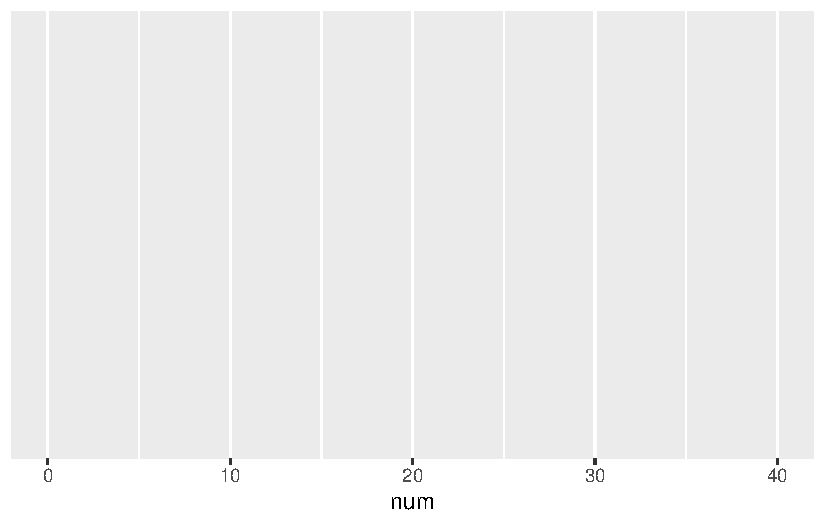
\includegraphics[keepaspectratio]{SVtilden_Code_emmaedit_files/figure-pdf/unnamed-chunk-5-1.pdf}}

\begin{Shaded}
\begin{Highlighting}[]
  \FunctionTok{geom\_histogram}\NormalTok{()}
\end{Highlighting}
\end{Shaded}

\begin{verbatim}
geom_bar: na.rm = FALSE, orientation = NA, lineend = butt, linejoin = mitre
stat_bin: na.rm = FALSE, binwidth = NULL, bins = NULL, orientation = NA
position_stack 
\end{verbatim}

\begin{Shaded}
\begin{Highlighting}[]
\CommentTok{\#HISTOGRAM FOR DISTRIBUTION OF TEMP DIFFERENCE}
\FunctionTok{library}\NormalTok{(dplyr)}
\FunctionTok{library}\NormalTok{(ggplot2)}

\NormalTok{tempdiffbymoisture }\SpecialCharTok{\%\textgreater{}\%}
  \FunctionTok{filter}\NormalTok{(PP }\SpecialCharTok{==} \DecValTok{1}\NormalTok{) }\SpecialCharTok{\%\textgreater{}\%}
  \FunctionTok{ggplot}\NormalTok{(}\FunctionTok{aes}\NormalTok{(}\AttributeTok{x =}\NormalTok{ diff\_H\_C)) }\SpecialCharTok{+}
  \FunctionTok{geom\_histogram}\NormalTok{(}\AttributeTok{binwidth =} \FloatTok{0.5}\NormalTok{, }\AttributeTok{fill =} \StringTok{"lightblue"}\NormalTok{, }\AttributeTok{color =} \StringTok{"black"}\NormalTok{, }\AttributeTok{alpha =} \FloatTok{0.7}\NormalTok{) }\SpecialCharTok{+}
  \FunctionTok{facet\_wrap}\NormalTok{(}\SpecialCharTok{\textasciitilde{}}\NormalTok{ depth) }\SpecialCharTok{+}
  \FunctionTok{labs}\NormalTok{(}
    \AttributeTok{x =} \StringTok{"Temperature Difference (Heated {-} Control)"}\NormalTok{,}
    \AttributeTok{y =} \StringTok{"Frequency"}\NormalTok{,}
    \AttributeTok{title =} \StringTok{"Temp Diff (PP = 1)"}
\NormalTok{  ) }\SpecialCharTok{+}
  \FunctionTok{theme}\NormalTok{(}
    \AttributeTok{strip.text =} \FunctionTok{element\_text}\NormalTok{(}\AttributeTok{size =} \DecValTok{12}\NormalTok{, }\AttributeTok{face =} \StringTok{"italic"}\NormalTok{),}
    \AttributeTok{axis.text =} \FunctionTok{element\_text}\NormalTok{(}\AttributeTok{size =} \DecValTok{10}\NormalTok{),}
    \AttributeTok{axis.title =} \FunctionTok{element\_text}\NormalTok{(}\AttributeTok{size =} \DecValTok{12}\NormalTok{),}
    \AttributeTok{plot.title =} \FunctionTok{element\_text}\NormalTok{(}\AttributeTok{size =} \DecValTok{14}\NormalTok{, }\AttributeTok{face =} \StringTok{"bold"}\NormalTok{)}
\NormalTok{  )}
\end{Highlighting}
\end{Shaded}

\pandocbounded{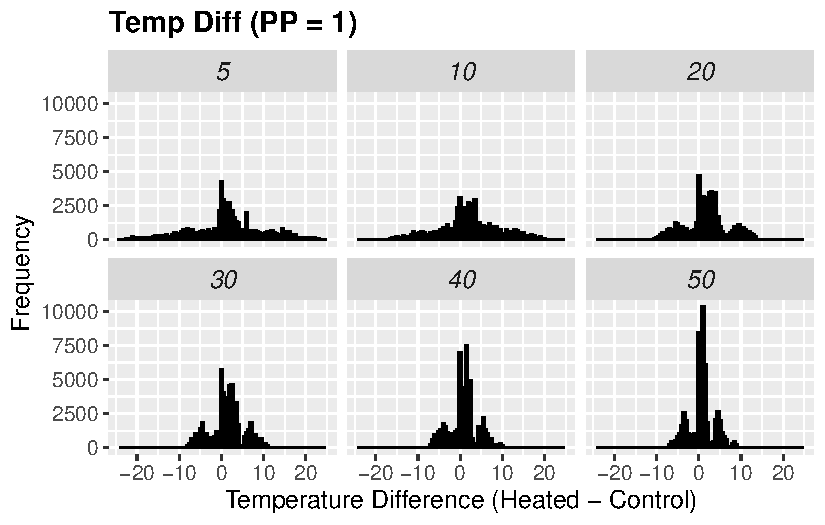
\includegraphics[keepaspectratio]{SVtilden_Code_emmaedit_files/figure-pdf/unnamed-chunk-6-1.pdf}}

\begin{Shaded}
\begin{Highlighting}[]
\CommentTok{\# KEEP}
\CommentTok{\#Raw Temp data SoilVUE}
\FunctionTok{ggplot}\NormalTok{(temp\_filtered\_Burned, }\FunctionTok{aes}\NormalTok{(}\AttributeTok{x =}\NormalTok{ TIMESTAMP, }\AttributeTok{y =}\NormalTok{ num, }\AttributeTok{color =}\NormalTok{ trt)) }\SpecialCharTok{+}
  \FunctionTok{geom\_point}\NormalTok{(}\AttributeTok{shape =} \DecValTok{16}\NormalTok{, }\AttributeTok{size =} \DecValTok{1}\NormalTok{) }\SpecialCharTok{+} 
  \FunctionTok{ylab}\NormalTok{(}\FunctionTok{expression}\NormalTok{(}\StringTok{"Temperature (degree*C)"}\NormalTok{)) }\SpecialCharTok{+}
  \FunctionTok{xlab}\NormalTok{(}\StringTok{"Date"}\NormalTok{) }\SpecialCharTok{+}
  \FunctionTok{theme\_bw}\NormalTok{() }\SpecialCharTok{+}
  \FunctionTok{theme}\NormalTok{(}
    \AttributeTok{legend.text =} \FunctionTok{element\_text}\NormalTok{(}\AttributeTok{size=}\DecValTok{14}\NormalTok{),}
    \AttributeTok{axis.text.x =} \FunctionTok{element\_text}\NormalTok{(}\AttributeTok{size=} \DecValTok{14}\NormalTok{, }\AttributeTok{angle =} \SpecialCharTok{{-}}\DecValTok{45}\NormalTok{, }\AttributeTok{vjust =} \FloatTok{0.5}\NormalTok{),}
    \AttributeTok{axis.text.y =} \FunctionTok{element\_text}\NormalTok{(}\AttributeTok{size =} \DecValTok{14}\NormalTok{),}
    \AttributeTok{axis.title.x =} \FunctionTok{element\_text}\NormalTok{(}\AttributeTok{size=}\DecValTok{14}\NormalTok{),  }\CommentTok{\# Increase x{-}axis label font size}
    \AttributeTok{axis.title.y =} \FunctionTok{element\_text}\NormalTok{(}\AttributeTok{size=}\DecValTok{14}\NormalTok{),  }\CommentTok{\# Increase y{-}axis label font size}
    \AttributeTok{strip.text =} \FunctionTok{element\_text}\NormalTok{(}\AttributeTok{size =} \DecValTok{12}\NormalTok{, }\AttributeTok{color =} \StringTok{"black"}\NormalTok{, }\AttributeTok{face =} \StringTok{"italic"}\NormalTok{),}
    \AttributeTok{legend.title =} \FunctionTok{element\_blank}\NormalTok{()  }\CommentTok{\# Remove legend title}
\NormalTok{  ) }\SpecialCharTok{+}
  \FunctionTok{guides}\NormalTok{(}\AttributeTok{color =} \FunctionTok{guide\_legend}\NormalTok{(}\AttributeTok{title =} \ConstantTok{FALSE}\NormalTok{)) }\SpecialCharTok{+}  \CommentTok{\# Remove legend title}
  \FunctionTok{facet\_grid}\NormalTok{(PP }\SpecialCharTok{\textasciitilde{}}\NormalTok{ depth) }\SpecialCharTok{+}
  \FunctionTok{ggtitle}\NormalTok{(}\StringTok{"SoilVUE Controlled and Heated Temperature Burned Plots 1{-}4"}\NormalTok{) }\SpecialCharTok{+}
  \FunctionTok{scale\_color\_manual}\NormalTok{(}\AttributeTok{values =} \FunctionTok{c}\NormalTok{(}\StringTok{"red"}\NormalTok{,}\StringTok{"blue"}\NormalTok{))}
\end{Highlighting}
\end{Shaded}

\begin{verbatim}
Warning: Removed 1725 rows containing missing values or values outside the scale range
(`geom_point()`).
\end{verbatim}

\pandocbounded{\includegraphics[keepaspectratio]{SVtilden_Code_emmaedit_files/figure-pdf/unnamed-chunk-7-1.pdf}}

\section{Plot 1 heated}\label{plot-1-heated}

\begin{Shaded}
\begin{Highlighting}[]
\CommentTok{\#Only for plot one because we only heated PP 1}
\FunctionTok{ggplot}\NormalTok{(temp\_filtered\_Burned, }
       \FunctionTok{aes}\NormalTok{(}\AttributeTok{x =}\NormalTok{ TIMESTAMP, }\AttributeTok{y =}\NormalTok{ num, }\AttributeTok{color =}\NormalTok{ trt)) }\SpecialCharTok{+}
  \FunctionTok{geom\_point}\NormalTok{(}\AttributeTok{shape =} \DecValTok{16}\NormalTok{, }\AttributeTok{size =} \DecValTok{1}\NormalTok{) }\SpecialCharTok{+} 
  \FunctionTok{ylab}\NormalTok{(}\FunctionTok{expression}\NormalTok{(}\StringTok{"Temperature (degree*C)"}\NormalTok{)) }\SpecialCharTok{+}
  \FunctionTok{xlab}\NormalTok{(}\StringTok{"Date"}\NormalTok{) }\SpecialCharTok{+}
  \FunctionTok{theme\_bw}\NormalTok{() }\SpecialCharTok{+}
  \FunctionTok{theme}\NormalTok{(}
    \AttributeTok{legend.text =} \FunctionTok{element\_text}\NormalTok{(}\AttributeTok{size=}\DecValTok{14}\NormalTok{),}
    \AttributeTok{axis.text.x =} \FunctionTok{element\_text}\NormalTok{(}\AttributeTok{size=}\DecValTok{14}\NormalTok{, }\AttributeTok{angle =} \SpecialCharTok{{-}}\DecValTok{45}\NormalTok{, }\AttributeTok{vjust =} \FloatTok{0.5}\NormalTok{),}
    \AttributeTok{axis.text.y =} \FunctionTok{element\_text}\NormalTok{(}\AttributeTok{size=}\DecValTok{14}\NormalTok{),}
    \AttributeTok{axis.title.x =} \FunctionTok{element\_text}\NormalTok{(}\AttributeTok{size=}\DecValTok{14}\NormalTok{),}
    \AttributeTok{axis.title.y =} \FunctionTok{element\_text}\NormalTok{(}\AttributeTok{size=}\DecValTok{14}\NormalTok{),}
    \AttributeTok{strip.text =} \FunctionTok{element\_text}\NormalTok{(}\AttributeTok{size=}\DecValTok{12}\NormalTok{, }\AttributeTok{color=}\StringTok{"black"}\NormalTok{, }\AttributeTok{face=}\StringTok{"italic"}\NormalTok{),}
    \AttributeTok{legend.title =} \FunctionTok{element\_blank}\NormalTok{()}
\NormalTok{  ) }\SpecialCharTok{+}
  \FunctionTok{guides}\NormalTok{(}\AttributeTok{color =} \FunctionTok{guide\_legend}\NormalTok{(}\AttributeTok{title =} \ConstantTok{FALSE}\NormalTok{)) }\SpecialCharTok{+}
  \FunctionTok{facet\_wrap}\NormalTok{(. }\SpecialCharTok{\textasciitilde{}}\NormalTok{ depth, }\AttributeTok{ncol =} \DecValTok{1}\NormalTok{) }\SpecialCharTok{+}  \CommentTok{\# Only facet by depth now}
  \FunctionTok{ggtitle}\NormalTok{(}\StringTok{"SoilVUE Controlled and Heated Temperature Burned Plot 1"}\NormalTok{) }\SpecialCharTok{+}
  \FunctionTok{scale\_color\_manual}\NormalTok{(}\AttributeTok{values =} \FunctionTok{c}\NormalTok{(}\StringTok{"red"}\NormalTok{, }\StringTok{"blue"}\NormalTok{))}
\end{Highlighting}
\end{Shaded}

\begin{verbatim}
Warning: Removed 1725 rows containing missing values or values outside the scale range
(`geom_point()`).
\end{verbatim}

\pandocbounded{\includegraphics[keepaspectratio]{SVtilden_Code_emmaedit_files/figure-pdf/unnamed-chunk-8-1.pdf}}

\begin{Shaded}
\begin{Highlighting}[]
\CommentTok{\#Raw Temp data SoilVUE}
\FunctionTok{ggplot}\NormalTok{(temp\_filtered\_Unburned, }\FunctionTok{aes}\NormalTok{(}\AttributeTok{x =}\NormalTok{ TIMESTAMP, }\AttributeTok{y =}\NormalTok{ num, }\AttributeTok{color =}\NormalTok{ trt)) }\SpecialCharTok{+}
  \FunctionTok{geom\_point}\NormalTok{(}\AttributeTok{shape =} \DecValTok{16}\NormalTok{, }\AttributeTok{size =} \DecValTok{1}\NormalTok{) }\SpecialCharTok{+} 
  \FunctionTok{ylab}\NormalTok{(}\FunctionTok{expression}\NormalTok{(}\StringTok{"Temperature (degree*C)"}\NormalTok{)) }\SpecialCharTok{+}
  \FunctionTok{xlab}\NormalTok{(}\StringTok{"Date"}\NormalTok{) }\SpecialCharTok{+}
  \FunctionTok{theme\_bw}\NormalTok{() }\SpecialCharTok{+}
  \FunctionTok{theme}\NormalTok{(}
    \AttributeTok{legend.text =} \FunctionTok{element\_text}\NormalTok{(}\AttributeTok{size=}\DecValTok{14}\NormalTok{),}
    \AttributeTok{axis.text.x =} \FunctionTok{element\_text}\NormalTok{(}\AttributeTok{size=} \DecValTok{14}\NormalTok{, }\AttributeTok{angle =} \SpecialCharTok{{-}}\DecValTok{45}\NormalTok{, }\AttributeTok{vjust =} \FloatTok{0.5}\NormalTok{),}
    \AttributeTok{axis.text.y =} \FunctionTok{element\_text}\NormalTok{(}\AttributeTok{size =} \DecValTok{14}\NormalTok{),}
    \AttributeTok{axis.title.x =} \FunctionTok{element\_text}\NormalTok{(}\AttributeTok{size=}\DecValTok{14}\NormalTok{),  }\CommentTok{\# Increase x{-}axis label font size}
    \AttributeTok{axis.title.y =} \FunctionTok{element\_text}\NormalTok{(}\AttributeTok{size=}\DecValTok{14}\NormalTok{),  }\CommentTok{\# Increase y{-}axis label font size}
    \AttributeTok{strip.text =} \FunctionTok{element\_text}\NormalTok{(}\AttributeTok{size =} \DecValTok{12}\NormalTok{, }\AttributeTok{color =} \StringTok{"black"}\NormalTok{, }\AttributeTok{face =} \StringTok{"italic"}\NormalTok{),}
    \AttributeTok{legend.title =} \FunctionTok{element\_blank}\NormalTok{()  }\CommentTok{\# Remove legend title}
\NormalTok{  ) }\SpecialCharTok{+}
  \FunctionTok{guides}\NormalTok{(}\AttributeTok{color =} \FunctionTok{guide\_legend}\NormalTok{(}\AttributeTok{title =} \ConstantTok{FALSE}\NormalTok{)) }\SpecialCharTok{+}  \CommentTok{\# Remove legend title}
  \FunctionTok{facet\_grid}\NormalTok{(PP }\SpecialCharTok{\textasciitilde{}}\NormalTok{ depth) }\SpecialCharTok{+}
  \FunctionTok{ggtitle}\NormalTok{(}\StringTok{"SoilVUE Controlled Temperature Unburned Plots 1{-}4"}\NormalTok{) }\SpecialCharTok{+}
  \FunctionTok{scale\_color\_manual}\NormalTok{(}\AttributeTok{values =} \FunctionTok{c}\NormalTok{(}\StringTok{"red"}\NormalTok{,}\StringTok{"blue"}\NormalTok{))}
\end{Highlighting}
\end{Shaded}

\begin{verbatim}
Warning: Removed 864 rows containing missing values or values outside the scale range
(`geom_point()`).
\end{verbatim}

\pandocbounded{\includegraphics[keepaspectratio]{SVtilden_Code_emmaedit_files/figure-pdf/unnamed-chunk-9-1.pdf}}

\begin{Shaded}
\begin{Highlighting}[]
  \CommentTok{\#ggsave("C:/Program Files/RStudio/Tilden Park Warming/Graphs/SoilVUE Controlled Temperature Unburned Plots 1{-}4.jpg", width=15,height=10)}
\CommentTok{\# ggsave("C:/Program Files/RStudio/Task 5 Microwarming/Plots/Research Paper/SoilVUE Controlled and Heated Temperature Plots 1{-}3.jpg", width=15, height=10)}
\end{Highlighting}
\end{Shaded}

\begin{Shaded}
\begin{Highlighting}[]
\CommentTok{\# Temperature timeseries BH1}
\NormalTok{t\_h\_sv }\SpecialCharTok{|\textgreater{}}
  \FunctionTok{filter}\NormalTok{(PP }\SpecialCharTok{==} \DecValTok{1}\NormalTok{) }\SpecialCharTok{|\textgreater{}}
  \FunctionTok{ggplot}\NormalTok{(}\FunctionTok{aes}\NormalTok{(}\AttributeTok{x =}\NormalTok{ TIMESTAMP, }\AttributeTok{y =}\NormalTok{ num)) }\SpecialCharTok{+}
  \FunctionTok{geom\_point}\NormalTok{(}\AttributeTok{shape =} \DecValTok{16}\NormalTok{, }\AttributeTok{size =} \DecValTok{1}\NormalTok{, }\AttributeTok{color =} \StringTok{"red"}\NormalTok{) }\SpecialCharTok{+}
  \FunctionTok{ylab}\NormalTok{(}\FunctionTok{expression}\NormalTok{(}\StringTok{"Temperature (degree*C)"}\NormalTok{)) }\SpecialCharTok{+}
  \FunctionTok{xlab}\NormalTok{(}\StringTok{"Date"}\NormalTok{) }\SpecialCharTok{+}
  \FunctionTok{theme\_bw}\NormalTok{() }\SpecialCharTok{+}
  \FunctionTok{theme}\NormalTok{(}
    \AttributeTok{legend.text =} \FunctionTok{element\_text}\NormalTok{(}\AttributeTok{size=}\DecValTok{14}\NormalTok{),}
    \AttributeTok{axis.text.x =} \FunctionTok{element\_text}\NormalTok{(}\AttributeTok{size=} \DecValTok{14}\NormalTok{, }\AttributeTok{angle =} \SpecialCharTok{{-}}\DecValTok{45}\NormalTok{, }\AttributeTok{vjust =} \FloatTok{0.5}\NormalTok{),}
    \AttributeTok{axis.text.y =} \FunctionTok{element\_text}\NormalTok{(}\AttributeTok{size =} \DecValTok{14}\NormalTok{),}
    \AttributeTok{axis.title.x =} \FunctionTok{element\_text}\NormalTok{(}\AttributeTok{size=}\DecValTok{14}\NormalTok{),  }\CommentTok{\# Increase x{-}axis label font size}
    \AttributeTok{axis.title.y =} \FunctionTok{element\_text}\NormalTok{(}\AttributeTok{size=}\DecValTok{14}\NormalTok{),  }\CommentTok{\# Increase y{-}axis label font size}
    \AttributeTok{strip.text =} \FunctionTok{element\_text}\NormalTok{(}\AttributeTok{size =} \DecValTok{12}\NormalTok{, }\AttributeTok{color =} \StringTok{"black"}\NormalTok{, }\AttributeTok{face =} \StringTok{"italic"}\NormalTok{),}
    \AttributeTok{legend.title =} \FunctionTok{element\_blank}\NormalTok{()  }\CommentTok{\# Remove legend title}
\NormalTok{  ) }\SpecialCharTok{+}
  \FunctionTok{guides}\NormalTok{(}\AttributeTok{color =} \FunctionTok{guide\_legend}\NormalTok{(}\AttributeTok{title =} \ConstantTok{FALSE}\NormalTok{)) }\SpecialCharTok{+}  \CommentTok{\# Remove legend title}
  \FunctionTok{facet\_grid}\NormalTok{(}\SpecialCharTok{\textasciitilde{}}\NormalTok{ depth) }\SpecialCharTok{+}
  \FunctionTok{ggtitle}\NormalTok{(}\StringTok{"Temperature Timeseries Burned Heated Plot 1"}\NormalTok{)}
\end{Highlighting}
\end{Shaded}

\begin{verbatim}
Warning: Removed 216 rows containing missing values or values outside the scale range
(`geom_point()`).
\end{verbatim}

\pandocbounded{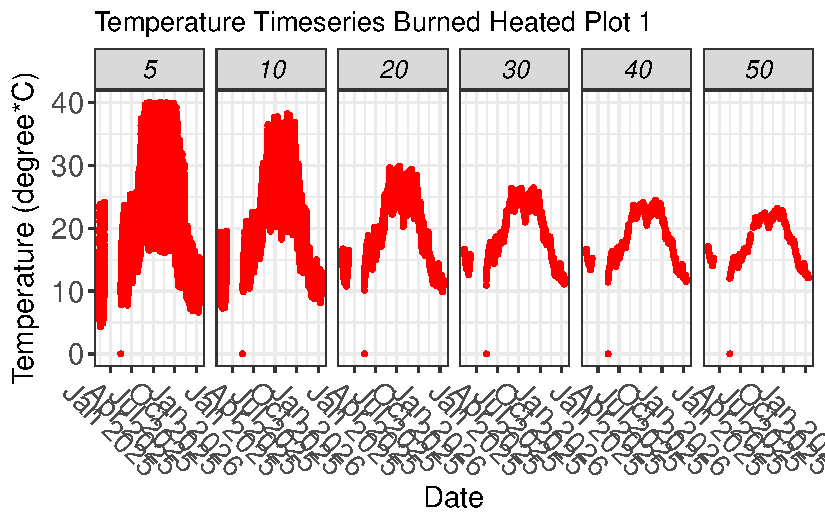
\includegraphics[keepaspectratio]{SVtilden_Code_emmaedit_files/figure-pdf/unnamed-chunk-10-1.pdf}}

\begin{Shaded}
\begin{Highlighting}[]
\NormalTok{t\_c\_sv }\SpecialCharTok{|\textgreater{}}
  \FunctionTok{filter}\NormalTok{(PP }\SpecialCharTok{==} \DecValTok{1}\NormalTok{) }\SpecialCharTok{|\textgreater{}}
  \FunctionTok{ggplot}\NormalTok{(}\FunctionTok{aes}\NormalTok{(}\AttributeTok{x =}\NormalTok{ TIMESTAMP, }\AttributeTok{y =}\NormalTok{ num)) }\SpecialCharTok{+}
  \FunctionTok{geom\_point}\NormalTok{(}\AttributeTok{shape =} \DecValTok{16}\NormalTok{, }\AttributeTok{size =} \DecValTok{1}\NormalTok{, }\AttributeTok{color =} \StringTok{"blue"}\NormalTok{) }\SpecialCharTok{+}
  \FunctionTok{ylab}\NormalTok{(}\FunctionTok{expression}\NormalTok{(}\StringTok{"Temperature (degree*C)"}\NormalTok{)) }\SpecialCharTok{+}
  \FunctionTok{xlab}\NormalTok{(}\StringTok{"Date"}\NormalTok{) }\SpecialCharTok{+}
  \FunctionTok{theme\_bw}\NormalTok{() }\SpecialCharTok{+}
  \FunctionTok{theme}\NormalTok{(}
    \AttributeTok{legend.text =} \FunctionTok{element\_text}\NormalTok{(}\AttributeTok{size=}\DecValTok{14}\NormalTok{),}
    \AttributeTok{axis.text.x =} \FunctionTok{element\_text}\NormalTok{(}\AttributeTok{size=} \DecValTok{14}\NormalTok{, }\AttributeTok{angle =} \SpecialCharTok{{-}}\DecValTok{45}\NormalTok{, }\AttributeTok{vjust =} \FloatTok{0.5}\NormalTok{),}
    \AttributeTok{axis.text.y =} \FunctionTok{element\_text}\NormalTok{(}\AttributeTok{size =} \DecValTok{14}\NormalTok{),}
    \AttributeTok{axis.title.x =} \FunctionTok{element\_text}\NormalTok{(}\AttributeTok{size=}\DecValTok{14}\NormalTok{),  }\CommentTok{\# Increase x{-}axis label font size}
    \AttributeTok{axis.title.y =} \FunctionTok{element\_text}\NormalTok{(}\AttributeTok{size=}\DecValTok{14}\NormalTok{),  }\CommentTok{\# Increase y{-}axis label font size}
    \AttributeTok{strip.text =} \FunctionTok{element\_text}\NormalTok{(}\AttributeTok{size =} \DecValTok{12}\NormalTok{, }\AttributeTok{color =} \StringTok{"black"}\NormalTok{, }\AttributeTok{face =} \StringTok{"italic"}\NormalTok{),}
    \AttributeTok{legend.title =} \FunctionTok{element\_blank}\NormalTok{()  }\CommentTok{\# Remove legend title}
\NormalTok{  ) }\SpecialCharTok{+}
  \FunctionTok{guides}\NormalTok{(}\AttributeTok{color =} \FunctionTok{guide\_legend}\NormalTok{(}\AttributeTok{title =} \ConstantTok{FALSE}\NormalTok{)) }\SpecialCharTok{+}  \CommentTok{\# Remove legend title}
  \FunctionTok{facet\_grid}\NormalTok{(}\SpecialCharTok{\textasciitilde{}}\NormalTok{ depth) }\SpecialCharTok{+}
  \FunctionTok{ggtitle}\NormalTok{(}\StringTok{"Temperature Timeseries Burned Control Plot 1"}\NormalTok{)}
\end{Highlighting}
\end{Shaded}

\begin{verbatim}
Warning: Removed 216 rows containing missing values or values outside the scale range
(`geom_point()`).
\end{verbatim}

\pandocbounded{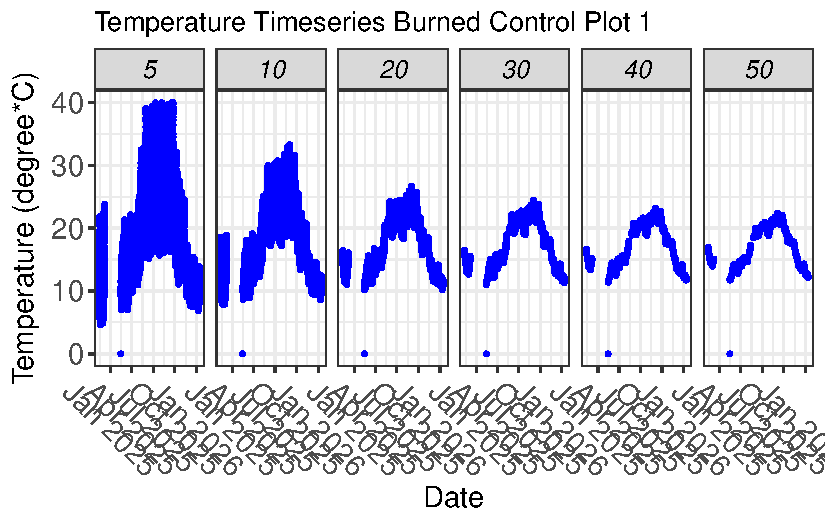
\includegraphics[keepaspectratio]{SVtilden_Code_emmaedit_files/figure-pdf/unnamed-chunk-10-2.pdf}}

\section{Summary statistics function and
calculations}\label{summary-statistics-function-and-calculations}

\begin{Shaded}
\begin{Highlighting}[]
\NormalTok{data\_summary }\OtherTok{\textless{}{-}} \ControlFlowTok{function}\NormalTok{(data, varname, groupnames)\{}
  \FunctionTok{require}\NormalTok{(plyr)}
\NormalTok{  summary\_func }\OtherTok{\textless{}{-}} \ControlFlowTok{function}\NormalTok{(x, col)\{}
    \FunctionTok{c}\NormalTok{(}\AttributeTok{mean =} \FunctionTok{mean}\NormalTok{(x[[col]], }\AttributeTok{na.rm=}\ConstantTok{TRUE}\NormalTok{),}
      \AttributeTok{sd =} \FunctionTok{sd}\NormalTok{(x[[col]], }\AttributeTok{na.rm=}\ConstantTok{TRUE}\NormalTok{))}
\NormalTok{  \}}
\NormalTok{  data\_sum}\OtherTok{\textless{}{-}}\FunctionTok{ddply}\NormalTok{(data, groupnames, }\AttributeTok{.fun=}\NormalTok{summary\_func,}
\NormalTok{                  varname)}
\NormalTok{  data\_sum }\OtherTok{\textless{}{-}} \FunctionTok{rename}\NormalTok{(data\_sum, }\FunctionTok{c}\NormalTok{(}\StringTok{"mean"} \OtherTok{=}\NormalTok{ varname))}
  \FunctionTok{return}\NormalTok{(data\_sum)}
\NormalTok{\}}

\CommentTok{\# Convert TIMESTAMP to datetime if it\textquotesingle{}s not already}
\NormalTok{temp.sv}\SpecialCharTok{$}\NormalTok{TIMESTAMP }\OtherTok{\textless{}{-}} \FunctionTok{as.POSIXct}\NormalTok{(temp.sv}\SpecialCharTok{$}\NormalTok{TIMESTAMP)}

\CommentTok{\# Ensure depth, trt, and PP are factors if they are categorical}
\NormalTok{temp.sv}\SpecialCharTok{$}\NormalTok{depth }\OtherTok{\textless{}{-}} \FunctionTok{as.factor}\NormalTok{(temp.sv}\SpecialCharTok{$}\NormalTok{depth)}
\NormalTok{temp.sv}\SpecialCharTok{$}\NormalTok{trt }\OtherTok{\textless{}{-}} \FunctionTok{as.factor}\NormalTok{(temp.sv}\SpecialCharTok{$}\NormalTok{trt)}
\NormalTok{temp.sv}\SpecialCharTok{$}\NormalTok{PP }\OtherTok{\textless{}{-}} \FunctionTok{as.factor}\NormalTok{(temp.sv}\SpecialCharTok{$}\NormalTok{PP)}

\CommentTok{\# Step 1: Calculate summary statistics for each group}
\NormalTok{summary\_sv }\OtherTok{\textless{}{-}}\NormalTok{ temp.sv }\SpecialCharTok{\%\textgreater{}\%}
\NormalTok{  dplyr}\SpecialCharTok{::}\FunctionTok{group\_by}\NormalTok{(TIMESTAMP, depth, trt, PP) }\SpecialCharTok{\%\textgreater{}\%}
\NormalTok{  dplyr}\SpecialCharTok{::}\FunctionTok{summarise}\NormalTok{(}
    \AttributeTok{num =} \FunctionTok{mean}\NormalTok{(num, }\AttributeTok{na.rm =} \ConstantTok{TRUE}\NormalTok{),  }\CommentTok{\# Calculate mean of \textquotesingle{}num\textquotesingle{} within each group}
\NormalTok{  )}
\end{Highlighting}
\end{Shaded}

\begin{verbatim}
`summarise()` has grouped output by 'TIMESTAMP', 'depth', 'trt'. You can
override using the `.groups` argument.
\end{verbatim}

\begin{Shaded}
\begin{Highlighting}[]
\CommentTok{\# Step 2: Calculate overall mean, sd, and se values per group (TIMESTAMP, depth, trt)}
\NormalTok{summary\_final\_sv }\OtherTok{\textless{}{-}}\NormalTok{ summary\_sv }\SpecialCharTok{\%\textgreater{}\%}
\NormalTok{  dplyr}\SpecialCharTok{::}\FunctionTok{group\_by}\NormalTok{(TIMESTAMP, depth, trt) }\SpecialCharTok{\%\textgreater{}\%}
\NormalTok{  dplyr}\SpecialCharTok{::}\FunctionTok{summarise}\NormalTok{(}
    \AttributeTok{mean =} \FunctionTok{mean}\NormalTok{(num, }\AttributeTok{na.rm =} \ConstantTok{TRUE}\NormalTok{),  }\CommentTok{\# Calculate mean of \textquotesingle{}mean\textquotesingle{} within each group}
    \AttributeTok{sd =} \FunctionTok{sd}\NormalTok{(num, }\AttributeTok{na.rm =} \ConstantTok{TRUE}\NormalTok{),      }\CommentTok{\# Calculate sd of \textquotesingle{}num\textquotesingle{} within each group}
    \AttributeTok{se =} \FunctionTok{sd}\NormalTok{(num, }\AttributeTok{na.rm =} \ConstantTok{TRUE}\NormalTok{) }\SpecialCharTok{/} \FunctionTok{sqrt}\NormalTok{(}\FunctionTok{sum}\NormalTok{(}\SpecialCharTok{!}\FunctionTok{is.na}\NormalTok{(num)))  }\CommentTok{\# Calculate se of \textquotesingle{}num\textquotesingle{} within each group}
\NormalTok{  )}
\end{Highlighting}
\end{Shaded}

\begin{verbatim}
`summarise()` has grouped output by 'TIMESTAMP', 'depth'. You can override
using the `.groups` argument.
\end{verbatim}

\begin{Shaded}
\begin{Highlighting}[]
\CommentTok{\# ...existing code...}

\CommentTok{\# {-}{-}{-} REPLACE from line \textasciitilde{}356: paired diffs between burned (PP 1{-}4) and unburned (PP 5{-}8) {-}{-}{-}}
\NormalTok{paired\_diff\_pp }\OtherTok{\textless{}{-}}\NormalTok{ temp.sv }\SpecialCharTok{\%\textgreater{}\%}
  \FunctionTok{filter}\NormalTok{(PP }\SpecialCharTok{\%in\%} \DecValTok{1}\SpecialCharTok{:}\DecValTok{8}\NormalTok{, }\SpecialCharTok{!}\FunctionTok{is.na}\NormalTok{(depth), }\SpecialCharTok{!}\FunctionTok{is.na}\NormalTok{(PP), }\SpecialCharTok{!}\FunctionTok{is.na}\NormalTok{(num)) }\SpecialCharTok{\%\textgreater{}\%}
  \FunctionTok{mutate}\NormalTok{(}
    \AttributeTok{pair =} \FunctionTok{if\_else}\NormalTok{(}\FunctionTok{as.integer}\NormalTok{(PP) }\SpecialCharTok{\textless{}=} \DecValTok{4}\NormalTok{L, }\FunctionTok{as.integer}\NormalTok{(PP), }\FunctionTok{as.integer}\NormalTok{(PP) }\SpecialCharTok{{-}} \DecValTok{4}\NormalTok{L),}
    \AttributeTok{side =} \FunctionTok{if\_else}\NormalTok{(}\FunctionTok{as.integer}\NormalTok{(PP) }\SpecialCharTok{\textless{}=} \DecValTok{4}\NormalTok{L, }\StringTok{"burned"}\NormalTok{, }\StringTok{"unburned"}\NormalTok{)}
\NormalTok{  ) }\SpecialCharTok{\%\textgreater{}\%}
  \FunctionTok{group\_by}\NormalTok{(TIMESTAMP, depth, pair, side) }\SpecialCharTok{\%\textgreater{}\%}
  \FunctionTok{summarise}\NormalTok{(}\AttributeTok{mean\_num =} \FunctionTok{mean}\NormalTok{(num, }\AttributeTok{na.rm =} \ConstantTok{TRUE}\NormalTok{), }\AttributeTok{.groups =} \StringTok{"drop"}\NormalTok{) }\SpecialCharTok{\%\textgreater{}\%}
  \FunctionTok{pivot\_wider}\NormalTok{(}\AttributeTok{names\_from =}\NormalTok{ side, }\AttributeTok{values\_from =}\NormalTok{ mean\_num) }\SpecialCharTok{\%\textgreater{}\%}
  \CommentTok{\# keep only pairs where both burned and unburned exist}
  \FunctionTok{filter}\NormalTok{(}\SpecialCharTok{!}\FunctionTok{is.na}\NormalTok{(burned) }\SpecialCharTok{\&} \SpecialCharTok{!}\FunctionTok{is.na}\NormalTok{(unburned)) }\SpecialCharTok{\%\textgreater{}\%}
  \FunctionTok{mutate}\NormalTok{(}
    \AttributeTok{diff\_burn\_unburn =}\NormalTok{ burned }\SpecialCharTok{{-}}\NormalTok{ unburned,}
    \AttributeTok{pair =} \FunctionTok{factor}\NormalTok{(pair),}
    \AttributeTok{depth =} \FunctionTok{factor}\NormalTok{(depth)}
\NormalTok{  ) }\SpecialCharTok{\%\textgreater{}\%}
  \FunctionTok{arrange}\NormalTok{(pair, depth, TIMESTAMP)}

\CommentTok{\# quick paired plot (keep y{-}limits {-}10..10)}
\NormalTok{p\_diff\_pp }\OtherTok{\textless{}{-}}\NormalTok{ paired\_diff\_pp }\SpecialCharTok{\%\textgreater{}\%}
  \FunctionTok{ggplot}\NormalTok{(}\FunctionTok{aes}\NormalTok{(}\AttributeTok{x =}\NormalTok{ TIMESTAMP, }\AttributeTok{y =}\NormalTok{ diff\_burn\_unburn, }\AttributeTok{group =}\NormalTok{ pair, }\AttributeTok{color =}\NormalTok{ pair)) }\SpecialCharTok{+}
  \FunctionTok{geom\_line}\NormalTok{(}\AttributeTok{size =} \FloatTok{0.6}\NormalTok{) }\SpecialCharTok{+}
  \FunctionTok{geom\_point}\NormalTok{(}\AttributeTok{size =} \DecValTok{1}\NormalTok{) }\SpecialCharTok{+}
  \FunctionTok{facet\_grid}\NormalTok{(pair }\SpecialCharTok{\textasciitilde{}}\NormalTok{ depth) }\SpecialCharTok{+}
  \FunctionTok{coord\_cartesian}\NormalTok{(}\AttributeTok{ylim =} \FunctionTok{c}\NormalTok{(}\SpecialCharTok{{-}}\DecValTok{10}\NormalTok{, }\DecValTok{10}\NormalTok{)) }\SpecialCharTok{+}
  \FunctionTok{labs}\NormalTok{(}\AttributeTok{x =} \StringTok{"Date"}\NormalTok{, }\AttributeTok{y =} \StringTok{"Temperature Difference (Burned {-} Unburned)"}\NormalTok{, }\AttributeTok{title =} \StringTok{"Paired Plot Temp Diff (burned vs unburned)"}\NormalTok{) }\SpecialCharTok{+}
  \FunctionTok{theme\_bw}\NormalTok{() }\SpecialCharTok{+}
  \FunctionTok{theme}\NormalTok{(}\AttributeTok{axis.text.x =} \FunctionTok{element\_text}\NormalTok{(}\AttributeTok{angle =} \SpecialCharTok{{-}}\DecValTok{45}\NormalTok{, }\AttributeTok{hjust =} \DecValTok{0}\NormalTok{))}
\end{Highlighting}
\end{Shaded}

\begin{verbatim}
Warning: Using `size` aesthetic for lines was deprecated in ggplot2 3.4.0.
i Please use `linewidth` instead.
\end{verbatim}

\begin{Shaded}
\begin{Highlighting}[]
\NormalTok{p\_diff\_pp}
\end{Highlighting}
\end{Shaded}

\begin{verbatim}
Warning: Removed 4 rows containing missing values or values outside the scale range
(`geom_line()`).
\end{verbatim}

\begin{verbatim}
Warning: Removed 24 rows containing missing values or values outside the scale range
(`geom_point()`).
\end{verbatim}

\pandocbounded{\includegraphics[keepaspectratio]{SVtilden_Code_emmaedit_files/figure-pdf/unnamed-chunk-12-1.pdf}}

\begin{Shaded}
\begin{Highlighting}[]
\CommentTok{\# ...existing code...}
\end{Highlighting}
\end{Shaded}

\section{Temp Difference between Burned and
Unburned}\label{temp-difference-between-burned-and-unburned}

\begin{Shaded}
\begin{Highlighting}[]
\CommentTok{\# Compute paired differences between H and C treatments within the same PP}
\CommentTok{\# pivot so H and C are side{-}by{-}side and compute difference}
\NormalTok{paired\_diff\_df }\OtherTok{\textless{}{-}}\NormalTok{ temp.sv }\SpecialCharTok{\%\textgreater{}\%}
  \FunctionTok{filter}\NormalTok{(}\SpecialCharTok{!}\FunctionTok{is.na}\NormalTok{(PP) }\SpecialCharTok{\&} \SpecialCharTok{!}\FunctionTok{is.na}\NormalTok{(depth) }\SpecialCharTok{\&} \SpecialCharTok{!}\FunctionTok{is.na}\NormalTok{(trt)) }\SpecialCharTok{\%\textgreater{}\%}
  \FunctionTok{group\_by}\NormalTok{(TIMESTAMP, depth, PP, trt) }\SpecialCharTok{\%\textgreater{}\%}
  \FunctionTok{summarise}\NormalTok{(}\AttributeTok{mean\_num =} \FunctionTok{mean}\NormalTok{(num, }\AttributeTok{na.rm =} \ConstantTok{TRUE}\NormalTok{), }\AttributeTok{.groups =} \StringTok{"drop"}\NormalTok{) }\SpecialCharTok{\%\textgreater{}\%}
  \FunctionTok{pivot\_wider}\NormalTok{(}\AttributeTok{names\_from =}\NormalTok{ trt, }\AttributeTok{values\_from =}\NormalTok{ mean\_num, }\AttributeTok{names\_prefix =} \StringTok{"mean\_"}\NormalTok{) }\SpecialCharTok{\%\textgreater{}\%}
  \CommentTok{\# require both mean\_H and mean\_C to be present for a paired diff}
  \FunctionTok{filter}\NormalTok{(}\SpecialCharTok{!}\FunctionTok{is.na}\NormalTok{(mean\_H) }\SpecialCharTok{\&} \SpecialCharTok{!}\FunctionTok{is.na}\NormalTok{(mean\_C)) }\SpecialCharTok{\%\textgreater{}\%}
  \FunctionTok{mutate}\NormalTok{(}
    \AttributeTok{diff\_num =}\NormalTok{ mean\_H }\SpecialCharTok{{-}}\NormalTok{ mean\_C,}
    \AttributeTok{PP =} \FunctionTok{factor}\NormalTok{(PP),}
    \AttributeTok{depth =} \FunctionTok{factor}\NormalTok{(depth)}
\NormalTok{  )}

\CommentTok{\# quick plot (paired diffs)}
\NormalTok{p\_diff }\OtherTok{\textless{}{-}}\NormalTok{ paired\_diff\_df }\SpecialCharTok{\%\textgreater{}\%}
  \FunctionTok{arrange}\NormalTok{(PP, depth, TIMESTAMP) }\SpecialCharTok{\%\textgreater{}\%}
  \FunctionTok{ggplot}\NormalTok{(}\FunctionTok{aes}\NormalTok{(}\AttributeTok{x =}\NormalTok{ TIMESTAMP, }\AttributeTok{y =}\NormalTok{ diff\_num, }\AttributeTok{group =}\NormalTok{ PP, }\AttributeTok{color =}\NormalTok{ PP)) }\SpecialCharTok{+}
  \FunctionTok{geom\_line}\NormalTok{(}\AttributeTok{size =} \FloatTok{0.6}\NormalTok{) }\SpecialCharTok{+}
  \FunctionTok{geom\_point}\NormalTok{(}\AttributeTok{size =} \DecValTok{1}\NormalTok{) }\SpecialCharTok{+}
  \FunctionTok{facet\_grid}\NormalTok{(PP }\SpecialCharTok{\textasciitilde{}}\NormalTok{ depth) }\SpecialCharTok{+}
  \FunctionTok{coord\_cartesian}\NormalTok{(}\AttributeTok{ylim =} \FunctionTok{c}\NormalTok{(}\SpecialCharTok{{-}}\DecValTok{10}\NormalTok{, }\DecValTok{10}\NormalTok{)) }\SpecialCharTok{+}
  \FunctionTok{labs}\NormalTok{(}\AttributeTok{x =} \StringTok{"Date"}\NormalTok{, }\AttributeTok{y =} \StringTok{"Temperature Difference (H {-} C)"}\NormalTok{, }\AttributeTok{title =} \StringTok{"Paired Plot Temperature Difference"}\NormalTok{) }\SpecialCharTok{+}
  \FunctionTok{theme\_bw}\NormalTok{() }\SpecialCharTok{+}
  \FunctionTok{theme}\NormalTok{(}\AttributeTok{axis.text.x =} \FunctionTok{element\_text}\NormalTok{(}\AttributeTok{angle =} \SpecialCharTok{{-}}\DecValTok{45}\NormalTok{, }\AttributeTok{hjust =} \DecValTok{0}\NormalTok{))}

\NormalTok{p\_diff}
\end{Highlighting}
\end{Shaded}

\begin{verbatim}
Warning: Removed 4 rows containing missing values or values outside the scale range
(`geom_line()`).
\end{verbatim}

\begin{verbatim}
Warning: Removed 24 rows containing missing values or values outside the scale range
(`geom_point()`).
\end{verbatim}

\pandocbounded{\includegraphics[keepaspectratio]{SVtilden_Code_emmaedit_files/figure-pdf/unnamed-chunk-13-1.pdf}}

\begin{Shaded}
\begin{Highlighting}[]
\CommentTok{\#MOISTURE DIFF BETWEEN BURNED AND UNBURNED}
\CommentTok{\# Step 1: Summarize Burned data}
\NormalTok{newburned }\OtherTok{\textless{}{-}}\NormalTok{ moisture\_filtered\_Burned }\SpecialCharTok{\%\textgreater{}\%} \FunctionTok{filter}\NormalTok{(trt }\SpecialCharTok{!=} \StringTok{"H"}\NormalTok{)}
\NormalTok{burned\_summary }\OtherTok{\textless{}{-}}\NormalTok{ newburned }\SpecialCharTok{\%\textgreater{}\%}
  \FunctionTok{group\_by}\NormalTok{(TIMESTAMP, depth) }\SpecialCharTok{\%\textgreater{}\%}
  \FunctionTok{summarize}\NormalTok{(}\AttributeTok{mean\_num\_burned =} \FunctionTok{mean}\NormalTok{(num, }\AttributeTok{na.rm =} \ConstantTok{TRUE}\NormalTok{), }\AttributeTok{.groups =} \StringTok{"drop"}\NormalTok{)}

\CommentTok{\# Step 2: Summarize Unburned data}
\NormalTok{unburned\_summary }\OtherTok{\textless{}{-}}\NormalTok{ moisture\_filtered\_Unburned }\SpecialCharTok{\%\textgreater{}\%}
  \FunctionTok{group\_by}\NormalTok{(TIMESTAMP, depth) }\SpecialCharTok{\%\textgreater{}\%}
  \FunctionTok{summarize}\NormalTok{(}\AttributeTok{mean\_num\_unburned =} \FunctionTok{mean}\NormalTok{(num, }\AttributeTok{na.rm =} \ConstantTok{TRUE}\NormalTok{), }\AttributeTok{.groups =} \StringTok{"drop"}\NormalTok{)}

\CommentTok{\# Step 3: Merge the two summaries by TIMESTAMP and Depth (inner join to get shared ones)}
\NormalTok{moist\_compare }\OtherTok{\textless{}{-}} \FunctionTok{inner\_join}\NormalTok{(burned\_summary, unburned\_summary, }\AttributeTok{by =} \FunctionTok{c}\NormalTok{(}\StringTok{"TIMESTAMP"}\NormalTok{, }\StringTok{"depth"}\NormalTok{))}

\CommentTok{\# Step 2: Reshape from wide to long format}
\NormalTok{long\_df }\OtherTok{\textless{}{-}}\NormalTok{ moist\_compare }\SpecialCharTok{\%\textgreater{}\%}
  \FunctionTok{pivot\_longer}\NormalTok{(}\AttributeTok{cols =} \FunctionTok{c}\NormalTok{(mean\_num\_burned, mean\_num\_unburned),}
               \AttributeTok{names\_to =} \StringTok{"condition"}\NormalTok{,}
               \AttributeTok{values\_to =} \StringTok{"mean\_moisture"}\NormalTok{) }\SpecialCharTok{\%\textgreater{}\%}
  \FunctionTok{mutate}\NormalTok{(}\AttributeTok{condition =} \FunctionTok{recode}\NormalTok{(condition,}
                            \AttributeTok{mean\_num\_burned =} \StringTok{"Burned"}\NormalTok{,}
                            \AttributeTok{mean\_num\_unburned =} \StringTok{"Unburned"}\NormalTok{))}

\CommentTok{\# Step 3: Plot burned and unburned on same plot}
\FunctionTok{ggplot}\NormalTok{(long\_df, }\FunctionTok{aes}\NormalTok{(}\AttributeTok{x =}\NormalTok{ TIMESTAMP, }\AttributeTok{y =}\NormalTok{ mean\_moisture, }\AttributeTok{color =}\NormalTok{ condition)) }\SpecialCharTok{+}
  \FunctionTok{geom\_line}\NormalTok{(}\AttributeTok{size =} \FloatTok{1.5}\NormalTok{) }\SpecialCharTok{+}
  \FunctionTok{facet\_wrap}\NormalTok{(}\SpecialCharTok{\textasciitilde{}}\NormalTok{ depth, }\AttributeTok{scales =} \StringTok{"free\_y"}\NormalTok{) }\SpecialCharTok{+}
  \FunctionTok{labs}\NormalTok{(}
    \AttributeTok{x =} \StringTok{"Timestamp"}\NormalTok{,}
    \AttributeTok{y =} \StringTok{"Mean Moisture"}\NormalTok{,}
    \AttributeTok{color =} \StringTok{"Condition"}
\NormalTok{  ) }\SpecialCharTok{+}
  \FunctionTok{theme\_minimal}\NormalTok{() }\SpecialCharTok{+}
  \FunctionTok{theme}\NormalTok{(}
    \AttributeTok{legend.text =} \FunctionTok{element\_text}\NormalTok{(}\AttributeTok{size=}\DecValTok{20}\NormalTok{),}
    \AttributeTok{legend.title =} \FunctionTok{element\_text}\NormalTok{(}\AttributeTok{size=}\DecValTok{20}\NormalTok{),}
    \AttributeTok{axis.text.x =} \FunctionTok{element\_text}\NormalTok{(}\AttributeTok{size=}\DecValTok{20}\NormalTok{, }\AttributeTok{angle =} \SpecialCharTok{{-}}\DecValTok{45}\NormalTok{, }\AttributeTok{vjust =} \FloatTok{0.5}\NormalTok{),}
    \AttributeTok{axis.text.y =} \FunctionTok{element\_text}\NormalTok{(}\AttributeTok{size=}\DecValTok{20}\NormalTok{),}
    \AttributeTok{axis.title.x =} \FunctionTok{element\_text}\NormalTok{(}\AttributeTok{size=}\DecValTok{20}\NormalTok{),}
    \AttributeTok{axis.title.y =} \FunctionTok{element\_text}\NormalTok{(}\AttributeTok{size=}\DecValTok{20}\NormalTok{),}
    \AttributeTok{strip.text =} \FunctionTok{element\_text}\NormalTok{(}\AttributeTok{size=}\DecValTok{18}\NormalTok{, }\AttributeTok{color=}\StringTok{"black"}\NormalTok{, }\AttributeTok{face=}\StringTok{"italic"}\NormalTok{)}
\NormalTok{  )}
\end{Highlighting}
\end{Shaded}

\begin{verbatim}
Warning: Removed 2 rows containing missing values or values outside the scale range
(`geom_line()`).
\end{verbatim}

\pandocbounded{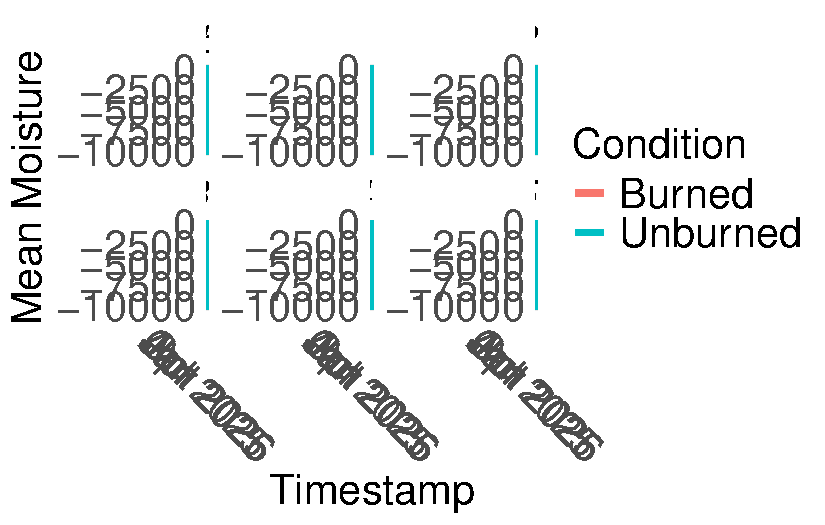
\includegraphics[keepaspectratio]{SVtilden_Code_emmaedit_files/figure-pdf/unnamed-chunk-14-1.pdf}}

\begin{Shaded}
\begin{Highlighting}[]
\CommentTok{\#standard deviation all depths}
\FunctionTok{ggplot}\NormalTok{(summary\_final\_sv, }\FunctionTok{aes}\NormalTok{(}\AttributeTok{x =}\NormalTok{ TIMESTAMP, }\AttributeTok{y =}\NormalTok{ mean, }\AttributeTok{colour =}\NormalTok{ trt)) }\SpecialCharTok{+}
  \FunctionTok{geom\_point}\NormalTok{(}\AttributeTok{size =} \FloatTok{0.5}\NormalTok{) }\SpecialCharTok{+}
  \FunctionTok{geom\_ribbon}\NormalTok{(}\FunctionTok{aes}\NormalTok{(}\AttributeTok{ymin =}\NormalTok{ mean }\SpecialCharTok{{-}}\NormalTok{ sd, }\AttributeTok{ymax =}\NormalTok{ mean }\SpecialCharTok{+}\NormalTok{ sd, }\AttributeTok{fill =}\NormalTok{ trt), }\AttributeTok{alpha =} \FloatTok{0.5}\NormalTok{, }\AttributeTok{colour =} \ConstantTok{NA}\NormalTok{) }\SpecialCharTok{+}
  \FunctionTok{scale\_color\_manual}\NormalTok{(}\AttributeTok{values =} \FunctionTok{c}\NormalTok{(}\StringTok{"C"} \OtherTok{=} \StringTok{"blue"}\NormalTok{, }\StringTok{"H"} \OtherTok{=} \StringTok{"red"}\NormalTok{)) }\SpecialCharTok{+}
  \FunctionTok{scale\_fill\_manual}\NormalTok{(}\AttributeTok{values =} \FunctionTok{c}\NormalTok{(}\StringTok{"C"} \OtherTok{=} \StringTok{"blue"}\NormalTok{, }\StringTok{"H"} \OtherTok{=} \StringTok{"red"}\NormalTok{)) }\SpecialCharTok{+}
  \FunctionTok{ylab}\NormalTok{(}\StringTok{"Mean Temp (degree*C)"}\NormalTok{) }\SpecialCharTok{+}
  \FunctionTok{xlab}\NormalTok{(}\StringTok{"Date"}\NormalTok{) }\SpecialCharTok{+}
  \FunctionTok{theme\_bw}\NormalTok{() }\SpecialCharTok{+}
  \FunctionTok{theme}\NormalTok{(}
    \AttributeTok{legend.text =} \FunctionTok{element\_text}\NormalTok{(}\AttributeTok{size=}\DecValTok{14}\NormalTok{),}
    \AttributeTok{axis.text.x =} \FunctionTok{element\_text}\NormalTok{(}\AttributeTok{size=} \DecValTok{14}\NormalTok{),}
    \AttributeTok{axis.text.y =} \FunctionTok{element\_text}\NormalTok{(}\AttributeTok{size =} \DecValTok{14}\NormalTok{),}
    \AttributeTok{axis.title.x =} \FunctionTok{element\_text}\NormalTok{(}\AttributeTok{size=}\DecValTok{14}\NormalTok{),  }\CommentTok{\# Increase x{-}axis label font size}
    \AttributeTok{axis.title.y =} \FunctionTok{element\_text}\NormalTok{(}\AttributeTok{size=}\DecValTok{14}\NormalTok{),}\CommentTok{\# Increase y{-}axis label font size}
    \AttributeTok{strip.text =} \FunctionTok{element\_text}\NormalTok{(}\AttributeTok{size =} \DecValTok{12}\NormalTok{, }\AttributeTok{color =} \StringTok{"black"}\NormalTok{, }\AttributeTok{face =} \StringTok{"italic"}\NormalTok{)}
\NormalTok{  ) }\SpecialCharTok{+}
  \FunctionTok{facet\_grid}\NormalTok{(}\SpecialCharTok{\textasciitilde{}}\NormalTok{depth) }\SpecialCharTok{+}
  \FunctionTok{ggtitle}\NormalTok{(}\StringTok{"SoilVUE Mean Temperature \& Standard Deviation Plots 1{-}3"}\NormalTok{) }\SpecialCharTok{+}
  \FunctionTok{scale\_x\_datetime}\NormalTok{(}\AttributeTok{breaks =} \StringTok{"8 days"}\NormalTok{, }\AttributeTok{date\_labels =} \StringTok{"\%b{-}\%d"}\NormalTok{) }\SpecialCharTok{+}
  \FunctionTok{theme}\NormalTok{(}\AttributeTok{axis.text.x =} \FunctionTok{element\_text}\NormalTok{(}\AttributeTok{angle =} \SpecialCharTok{{-}}\DecValTok{45}\NormalTok{)) }\SpecialCharTok{+}
  \FunctionTok{labs}\NormalTok{(}\AttributeTok{color =} \ConstantTok{NULL}\NormalTok{, }\AttributeTok{fill =} \ConstantTok{NULL}\NormalTok{)}
\end{Highlighting}
\end{Shaded}

\begin{verbatim}
Warning: Removed 12 rows containing missing values or values outside the scale range
(`geom_point()`).
\end{verbatim}

\begin{verbatim}
Warning: Removed 85 rows containing missing values or values outside the scale range
(`geom_ribbon()`).
\end{verbatim}

\pandocbounded{\includegraphics[keepaspectratio]{SVtilden_Code_emmaedit_files/figure-pdf/unnamed-chunk-15-1.pdf}}

\begin{Shaded}
\begin{Highlighting}[]
\CommentTok{\#KEEP }
\CommentTok{\#standard deviation plots 30 cm depth}
\NormalTok{summary\_final\_sv\_30cm }\OtherTok{\textless{}{-}} \FunctionTok{subset}\NormalTok{(summary\_final\_sv, depth }\SpecialCharTok{==} \StringTok{\textquotesingle{}30\textquotesingle{}}\NormalTok{)}

\FunctionTok{ggplot}\NormalTok{(summary\_final\_sv\_30cm, }\FunctionTok{aes}\NormalTok{(}\AttributeTok{x =}\NormalTok{ TIMESTAMP, }\AttributeTok{y =}\NormalTok{ mean, }\AttributeTok{colour =}\NormalTok{ trt)) }\SpecialCharTok{+}
  \FunctionTok{geom\_point}\NormalTok{(}\AttributeTok{size =} \FloatTok{0.5}\NormalTok{) }\SpecialCharTok{+}
  \FunctionTok{geom\_ribbon}\NormalTok{(}\FunctionTok{aes}\NormalTok{(}\AttributeTok{ymin =}\NormalTok{ mean }\SpecialCharTok{{-}}\NormalTok{ sd, }\AttributeTok{ymax =}\NormalTok{ mean }\SpecialCharTok{+}\NormalTok{ sd, }\AttributeTok{fill =}\NormalTok{ trt), }\AttributeTok{alpha =} \FloatTok{0.5}\NormalTok{, }\AttributeTok{colour =} \ConstantTok{NA}\NormalTok{) }\SpecialCharTok{+}
  \FunctionTok{scale\_color\_manual}\NormalTok{(}\AttributeTok{values =} \FunctionTok{c}\NormalTok{(}\StringTok{"C"} \OtherTok{=} \StringTok{"blue"}\NormalTok{, }\StringTok{"H"} \OtherTok{=} \StringTok{"red"}\NormalTok{)) }\SpecialCharTok{+}
  \FunctionTok{scale\_fill\_manual}\NormalTok{(}\AttributeTok{values =} \FunctionTok{c}\NormalTok{(}\StringTok{"C"} \OtherTok{=} \StringTok{"blue"}\NormalTok{, }\StringTok{"H"} \OtherTok{=} \StringTok{"red"}\NormalTok{)) }\SpecialCharTok{+}
  \FunctionTok{ylab}\NormalTok{(}\StringTok{"Temperature (degree*C)"}\NormalTok{) }\SpecialCharTok{+}
  \FunctionTok{xlab}\NormalTok{(}\StringTok{"Date"}\NormalTok{) }\SpecialCharTok{+}
  \FunctionTok{theme\_bw}\NormalTok{() }\SpecialCharTok{+}
  \FunctionTok{theme}\NormalTok{(}
    \AttributeTok{legend.text =} \FunctionTok{element\_text}\NormalTok{(}\AttributeTok{size=}\DecValTok{14}\NormalTok{),}
    \AttributeTok{axis.text.x =} \FunctionTok{element\_text}\NormalTok{(}\AttributeTok{size=} \DecValTok{14}\NormalTok{),}
    \AttributeTok{axis.text.y =} \FunctionTok{element\_text}\NormalTok{(}\AttributeTok{size =} \DecValTok{14}\NormalTok{),}
    \AttributeTok{axis.title.x =} \FunctionTok{element\_text}\NormalTok{(}\AttributeTok{size=}\DecValTok{14}\NormalTok{),  }\CommentTok{\# Increase x{-}axis label font size}
    \AttributeTok{axis.title.y =} \FunctionTok{element\_text}\NormalTok{(}\AttributeTok{size=}\DecValTok{14}\NormalTok{),}\CommentTok{\# Increase y{-}axis label font size}
    \AttributeTok{strip.text =} \FunctionTok{element\_text}\NormalTok{(}\AttributeTok{size =} \DecValTok{12}\NormalTok{, }\AttributeTok{color =} \StringTok{"black"}\NormalTok{, }\AttributeTok{face =} \StringTok{"italic"}\NormalTok{)}
\NormalTok{  ) }\SpecialCharTok{+}
  \FunctionTok{ggtitle}\NormalTok{(}\StringTok{"SoilVUE Temperature Standard Deviation Plot for 30 cm Depth"}\NormalTok{) }\SpecialCharTok{+}
  \FunctionTok{scale\_x\_datetime}\NormalTok{(}\AttributeTok{breaks =} \StringTok{"8 days"}\NormalTok{, }\AttributeTok{date\_labels =} \StringTok{"\%b{-}\%d"}\NormalTok{) }\SpecialCharTok{+}
  \FunctionTok{theme}\NormalTok{(}\AttributeTok{axis.text.x =} \FunctionTok{element\_text}\NormalTok{(}\AttributeTok{angle =} \SpecialCharTok{{-}}\DecValTok{45}\NormalTok{)) }\SpecialCharTok{+}
  \FunctionTok{labs}\NormalTok{(}\AttributeTok{color =} \ConstantTok{NULL}\NormalTok{, }\AttributeTok{fill =} \ConstantTok{NULL}\NormalTok{)}
\end{Highlighting}
\end{Shaded}

\begin{verbatim}
Warning: Removed 2 rows containing missing values or values outside the scale range
(`geom_point()`).
\end{verbatim}

\begin{verbatim}
Warning: Removed 2 rows containing missing values or values outside the scale range
(`geom_ribbon()`).
\end{verbatim}

\pandocbounded{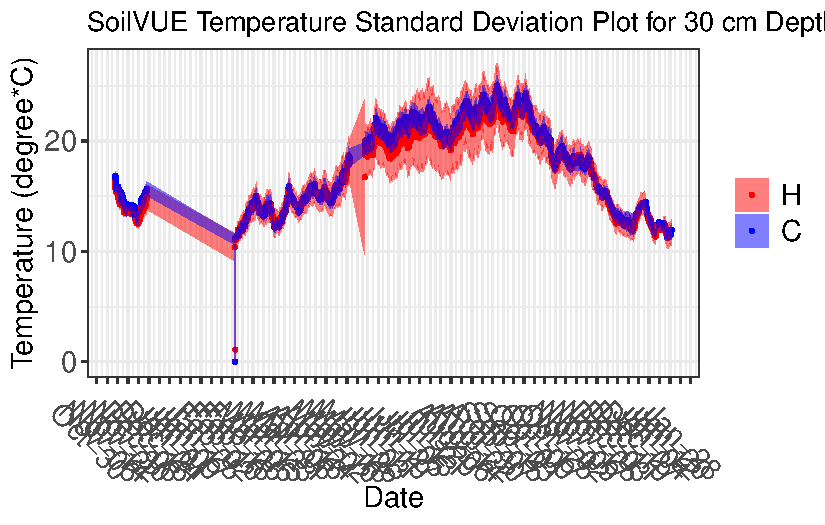
\includegraphics[keepaspectratio]{SVtilden_Code_emmaedit_files/figure-pdf/unnamed-chunk-16-1.pdf}}

\begin{Shaded}
\begin{Highlighting}[]
\CommentTok{\#Keep}
\CommentTok{\# moisture H and C (raw)}
\FunctionTok{ggplot}\NormalTok{(moisture.sv, }\FunctionTok{aes}\NormalTok{(}\AttributeTok{x=}\NormalTok{TIMESTAMP, }\AttributeTok{y=}\NormalTok{num, }\AttributeTok{colour=}\NormalTok{trt)) }\SpecialCharTok{+}
  \FunctionTok{geom\_point}\NormalTok{(}\AttributeTok{shape=}\DecValTok{16}\NormalTok{, }\AttributeTok{size=}\DecValTok{1}\NormalTok{) }\SpecialCharTok{+} 
  \FunctionTok{ylab}\NormalTok{(}\FunctionTok{expression}\NormalTok{(}\StringTok{"Moisture Content"}\NormalTok{)) }\SpecialCharTok{+}
  \FunctionTok{xlab}\NormalTok{(}\StringTok{"Date"}\NormalTok{) }\SpecialCharTok{+}
  \FunctionTok{scale\_color\_manual}\NormalTok{(}\AttributeTok{values =} \FunctionTok{c}\NormalTok{(}\StringTok{"C"} \OtherTok{=} \StringTok{"blue"}\NormalTok{, }\StringTok{"H"} \OtherTok{=} \StringTok{"red"}\NormalTok{)) }\SpecialCharTok{+}
  \FunctionTok{ggtitle}\NormalTok{(}\StringTok{"SoilVUE Moisture Plots 1{-}4"}\NormalTok{) }\SpecialCharTok{+}
  \FunctionTok{theme\_bw}\NormalTok{() }\SpecialCharTok{+}
  \FunctionTok{theme}\NormalTok{(}
    \AttributeTok{legend.text =} \FunctionTok{element\_text}\NormalTok{(}\AttributeTok{size=}\DecValTok{14}\NormalTok{),}
    \AttributeTok{axis.text.x =} \FunctionTok{element\_text}\NormalTok{(}\AttributeTok{size=} \DecValTok{14}\NormalTok{, }\AttributeTok{angle =} \SpecialCharTok{{-}}\DecValTok{45}\NormalTok{, }\AttributeTok{vjust =} \FloatTok{0.5}\NormalTok{),}
    \AttributeTok{axis.text.y =} \FunctionTok{element\_text}\NormalTok{(}\AttributeTok{size =} \DecValTok{14}\NormalTok{),}
    \AttributeTok{axis.title.x =} \FunctionTok{element\_text}\NormalTok{(}\AttributeTok{size=}\DecValTok{14}\NormalTok{),  }\CommentTok{\# Increase x{-}axis label font size}
    \AttributeTok{axis.title.y =} \FunctionTok{element\_text}\NormalTok{(}\AttributeTok{size=}\DecValTok{14}\NormalTok{),}\CommentTok{\# Increase y{-}axis label font size}
    \AttributeTok{strip.text =} \FunctionTok{element\_text}\NormalTok{(}\AttributeTok{size =} \DecValTok{12}\NormalTok{, }\AttributeTok{color =} \StringTok{"black"}\NormalTok{, }\AttributeTok{face =} \StringTok{"italic"}\NormalTok{)}
\NormalTok{  ) }\SpecialCharTok{+}
  \FunctionTok{guides}\NormalTok{(}\AttributeTok{colour =} \FunctionTok{guide\_legend}\NormalTok{(}\AttributeTok{title =} \ConstantTok{NULL}\NormalTok{)) }\SpecialCharTok{+}
  \FunctionTok{facet\_grid}\NormalTok{(PP}\SpecialCharTok{\textasciitilde{}}\NormalTok{depth)}
\end{Highlighting}
\end{Shaded}

\begin{verbatim}
Warning: Removed 2352 rows containing missing values or values outside the scale range
(`geom_point()`).
\end{verbatim}

\pandocbounded{\includegraphics[keepaspectratio]{SVtilden_Code_emmaedit_files/figure-pdf/unnamed-chunk-17-1.pdf}}

\begin{Shaded}
\begin{Highlighting}[]
  \CommentTok{\#ggsave("C:/Program Files/RStudio/Tilden Park Warming/Graphs/SoilVUE Moisture Plots 1{-}4.jpg", width=15,height=10)}
\CommentTok{\# ggsave("C:/Program Files/RStudio/Task 5 Microwarming/Plots/Research Paper/SoilVUE Moisture Plots 1{-}3.pdf.jpg", width=15, height=10)}

\FunctionTok{library}\NormalTok{(ggplot2)}

\CommentTok{\# Filter the data for PP 3}
\NormalTok{moisture.sv\_PP3 }\OtherTok{\textless{}{-}} \FunctionTok{subset}\NormalTok{(moisture.sv, PP }\SpecialCharTok{==} \DecValTok{3}\NormalTok{)}
\end{Highlighting}
\end{Shaded}

\begin{Shaded}
\begin{Highlighting}[]
\CommentTok{\#Keep }
\CommentTok{\# Create raw data plot 3}
\FunctionTok{ggplot}\NormalTok{(moisture.sv\_PP3, }\FunctionTok{aes}\NormalTok{(}\AttributeTok{x=}\NormalTok{TIMESTAMP, }\AttributeTok{y=}\NormalTok{num, }\AttributeTok{colour=}\NormalTok{trt)) }\SpecialCharTok{+}
  \FunctionTok{geom\_point}\NormalTok{(}\AttributeTok{shape=}\DecValTok{5}\NormalTok{, }\AttributeTok{size=}\FloatTok{0.5}\NormalTok{) }\SpecialCharTok{+} 
  \FunctionTok{ylab}\NormalTok{(}\FunctionTok{expression}\NormalTok{(}\StringTok{"Moisture Content"}\NormalTok{)) }\SpecialCharTok{+}
  \FunctionTok{xlab}\NormalTok{(}\StringTok{"Date"}\NormalTok{) }\SpecialCharTok{+}
  \FunctionTok{scale\_color\_manual}\NormalTok{(}\AttributeTok{values =} \FunctionTok{c}\NormalTok{(}\StringTok{"C"} \OtherTok{=} \StringTok{"blue"}\NormalTok{, }\StringTok{"H"} \OtherTok{=} \StringTok{"red"}\NormalTok{)) }\SpecialCharTok{+}
  \CommentTok{\#  scale\_x\_datetime(}
  \CommentTok{\#   date\_breaks = "10 days",       \# Set break intervals to 20 days}
  \CommentTok{\#    date\_labels = "\%d \%b"       \# Format the date labels}
  \CommentTok{\# ) +}
  \FunctionTok{ggtitle}\NormalTok{(}\StringTok{"SoilVUE Moisture Plot 3"}\NormalTok{) }\SpecialCharTok{+}
  \FunctionTok{theme\_bw}\NormalTok{() }\SpecialCharTok{+}
  \FunctionTok{theme}\NormalTok{(}
    \AttributeTok{legend.text =} \FunctionTok{element\_text}\NormalTok{(}\AttributeTok{size=}\DecValTok{14}\NormalTok{),}
    \AttributeTok{axis.text.x =} \FunctionTok{element\_text}\NormalTok{(}\AttributeTok{size=} \DecValTok{12}\NormalTok{, }\AttributeTok{angle =} \SpecialCharTok{{-}}\DecValTok{45}\NormalTok{, }\AttributeTok{vjust =} \FloatTok{0.5}\NormalTok{),}
    \AttributeTok{axis.text.y =} \FunctionTok{element\_text}\NormalTok{(}\AttributeTok{size =} \DecValTok{14}\NormalTok{),}
    \AttributeTok{axis.title.x =} \FunctionTok{element\_text}\NormalTok{(}\AttributeTok{size=}\DecValTok{14}\NormalTok{),  }\CommentTok{\# Increase x{-}axis label font size}
    \AttributeTok{axis.title.y =} \FunctionTok{element\_text}\NormalTok{(}\AttributeTok{size=}\DecValTok{14}\NormalTok{),}\CommentTok{\# Increase y{-}axis label font size}
    \AttributeTok{strip.text =} \FunctionTok{element\_text}\NormalTok{(}\AttributeTok{size =} \DecValTok{12}\NormalTok{, }\AttributeTok{color =} \StringTok{"black"}\NormalTok{, }\AttributeTok{face =} \StringTok{"italic"}\NormalTok{)}
\NormalTok{  ) }\SpecialCharTok{+}
  \FunctionTok{guides}\NormalTok{(}\AttributeTok{colour =} \FunctionTok{guide\_legend}\NormalTok{(}\AttributeTok{title =} \ConstantTok{NULL}\NormalTok{)) }\SpecialCharTok{+}
  \FunctionTok{facet\_grid}\NormalTok{(. }\SpecialCharTok{\textasciitilde{}}\NormalTok{ depth)}
\end{Highlighting}
\end{Shaded}

\begin{verbatim}
Warning: Removed 402 rows containing missing values or values outside the scale range
(`geom_point()`).
\end{verbatim}

\pandocbounded{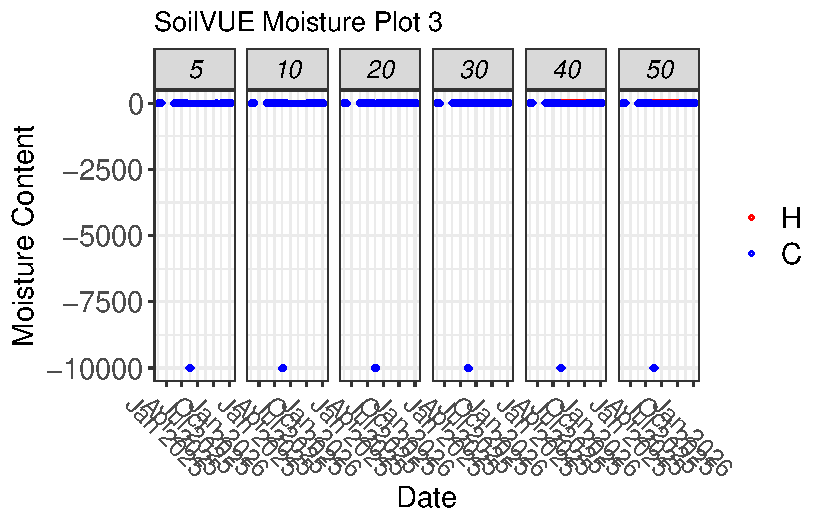
\includegraphics[keepaspectratio]{SVtilden_Code_emmaedit_files/figure-pdf/unnamed-chunk-18-1.pdf}}

\begin{Shaded}
\begin{Highlighting}[]
\CommentTok{\# ggsave("C:/Program Files/RStudio/Task 5 Microwarming/Plots/SoilVUE Moisture Plot 3.pdf", width=10, height=5)}
\CommentTok{\# ggsave("C:/Program Files/RStudio/Task 5 Microwarming/Plots/SoilVUE Moisture Plot 3.jpg", width=10, height=5)}


\NormalTok{moisture\_num }\OtherTok{\textless{}{-}}\NormalTok{ moisture.sv}\SpecialCharTok{$}\NormalTok{num}

\FunctionTok{names}\NormalTok{(temp.sv) }\OtherTok{\textless{}{-}} \FunctionTok{c}\NormalTok{(}\StringTok{"TIMESTAMP"}\NormalTok{, }\StringTok{"variable"}\NormalTok{, }\StringTok{"temp\_num"}\NormalTok{, }\StringTok{"plot"}\NormalTok{, }\StringTok{"depth"}\NormalTok{, }\StringTok{"avg"}\NormalTok{, }\StringTok{"PP"}\NormalTok{, }\StringTok{"trt"}\NormalTok{, }\StringTok{"measurement"}\NormalTok{)}

\NormalTok{temp\_moisture\_sv }\OtherTok{\textless{}{-}} \FunctionTok{cbind}\NormalTok{(temp.sv, }\AttributeTok{moisture\_num =}\NormalTok{ moisture.sv}\SpecialCharTok{$}\NormalTok{num)}
\end{Highlighting}
\end{Shaded}

\begin{verbatim}
Warning in as.data.table.list(x, keep.rownames = keep.rownames, check.names =
check.names, : Item 1 has 1219048 rows but longest item has 1273941; recycled
with remainder.
\end{verbatim}

\begin{Shaded}
\begin{Highlighting}[]
\CommentTok{\#Keep }
\CommentTok{\# Temp vs moisture }
\FunctionTok{ggplot}\NormalTok{(temp\_moisture\_sv, }\FunctionTok{aes}\NormalTok{(}\AttributeTok{x =}\NormalTok{ temp\_num, }\AttributeTok{y =}\NormalTok{ moisture\_num, }\AttributeTok{colour =}\NormalTok{ trt)) }\SpecialCharTok{+}
  \FunctionTok{geom\_point}\NormalTok{(}\AttributeTok{shape =} \DecValTok{1}\NormalTok{, }\AttributeTok{size =} \FloatTok{0.75}\NormalTok{) }\SpecialCharTok{+}
  \FunctionTok{ylab}\NormalTok{(}\FunctionTok{expression}\NormalTok{(}\StringTok{"Soil Moisture"}\NormalTok{)) }\SpecialCharTok{+}
  \FunctionTok{xlab}\NormalTok{(}\StringTok{"Temperature (degree*C)"}\NormalTok{) }\SpecialCharTok{+}
  \FunctionTok{labs}\NormalTok{(}\AttributeTok{title =} \StringTok{"SoilVUE Temperature vs Moisture Plots 1{-}3"}\NormalTok{) }\SpecialCharTok{+}
  \FunctionTok{theme\_bw}\NormalTok{() }\SpecialCharTok{+}
  \FunctionTok{facet\_grid}\NormalTok{(PP }\SpecialCharTok{\textasciitilde{}}\NormalTok{ depth) }\SpecialCharTok{+}
  \FunctionTok{scale\_color\_manual}\NormalTok{(}\AttributeTok{values =} \FunctionTok{c}\NormalTok{(}\StringTok{"C"} \OtherTok{=} \StringTok{"blue"}\NormalTok{, }\StringTok{"H"} \OtherTok{=} \StringTok{"red"}\NormalTok{))}
\end{Highlighting}
\end{Shaded}

\pandocbounded{\includegraphics[keepaspectratio]{SVtilden_Code_emmaedit_files/figure-pdf/unnamed-chunk-18-2.pdf}}

\begin{Shaded}
\begin{Highlighting}[]
\CommentTok{\# ggsave("C:/Program Files/RStudio/Task 5 Microwarming/Plots/SoilVUE Temperature vs Moisture Plots 1{-}3.pdf", width=15,height=10,dpi=300)}


\NormalTok{summary.moisture2 }\OtherTok{\textless{}{-}}\NormalTok{ moisture.sv }\SpecialCharTok{\%\textgreater{}\%}
\NormalTok{  dplyr}\SpecialCharTok{::}\FunctionTok{group\_by}\NormalTok{(TIMESTAMP,depth, trt) }\SpecialCharTok{\%\textgreater{}\%}
\NormalTok{  dplyr}\SpecialCharTok{::}\FunctionTok{summarise}\NormalTok{(}
    \AttributeTok{N=}\FunctionTok{length}\NormalTok{(num),}
    \AttributeTok{mean=} \FunctionTok{mean}\NormalTok{(num, }\AttributeTok{na.rm=}\NormalTok{T),}
    \AttributeTok{sd=}\FunctionTok{sd}\NormalTok{(num, }\AttributeTok{na.rm=}\NormalTok{T),}
    \AttributeTok{se=}\FunctionTok{sd}\NormalTok{(num, }\AttributeTok{na.rm=}\NormalTok{T)}\SpecialCharTok{/}\FunctionTok{sqrt}\NormalTok{(}\FunctionTok{sum}\NormalTok{(}\SpecialCharTok{!}\FunctionTok{is.na}\NormalTok{(num))))}
\end{Highlighting}
\end{Shaded}

\begin{verbatim}
`summarise()` has grouped output by 'TIMESTAMP', 'depth'. You can override
using the `.groups` argument.
\end{verbatim}

\begin{Shaded}
\begin{Highlighting}[]
\CommentTok{\#KEEP}
\CommentTok{\#standard deviation moisture }
\FunctionTok{ggplot}\NormalTok{(summary.moisture2, }\FunctionTok{aes}\NormalTok{(}\AttributeTok{x =}\NormalTok{ TIMESTAMP, }\AttributeTok{y =}\NormalTok{ mean, }\AttributeTok{colour =}\NormalTok{ trt)) }\SpecialCharTok{+}
  \FunctionTok{geom\_point}\NormalTok{(}\AttributeTok{size =} \DecValTok{1}\NormalTok{) }\SpecialCharTok{+}
  \FunctionTok{geom\_ribbon}\NormalTok{(}\FunctionTok{aes}\NormalTok{(}\AttributeTok{ymin =}\NormalTok{ mean }\SpecialCharTok{{-}}\NormalTok{ sd, }\AttributeTok{ymax =}\NormalTok{ mean }\SpecialCharTok{+}\NormalTok{ sd, }\AttributeTok{fill =}\NormalTok{ trt), }\AttributeTok{alpha =} \FloatTok{0.5}\NormalTok{, }\AttributeTok{colour =} \ConstantTok{NA}\NormalTok{) }\SpecialCharTok{+}
  \FunctionTok{scale\_color\_manual}\NormalTok{(}\AttributeTok{values =} \FunctionTok{c}\NormalTok{(}\StringTok{"C"} \OtherTok{=} \StringTok{"blue"}\NormalTok{, }\StringTok{"H"} \OtherTok{=} \StringTok{"red"}\NormalTok{)) }\SpecialCharTok{+}
  \FunctionTok{scale\_fill\_manual}\NormalTok{(}\AttributeTok{values =} \FunctionTok{c}\NormalTok{(}\StringTok{"C"} \OtherTok{=} \StringTok{"blue"}\NormalTok{, }\StringTok{"H"} \OtherTok{=} \StringTok{"red"}\NormalTok{)) }\SpecialCharTok{+}
  \FunctionTok{ylab}\NormalTok{(}\StringTok{"Moisture Content"}\NormalTok{) }\SpecialCharTok{+}
  \FunctionTok{xlab}\NormalTok{(}\StringTok{"Date"}\NormalTok{) }\SpecialCharTok{+}
  \FunctionTok{theme\_bw}\NormalTok{() }\SpecialCharTok{+}
  \FunctionTok{theme}\NormalTok{(}
    \AttributeTok{legend.text =} \FunctionTok{element\_text}\NormalTok{(}\AttributeTok{size=}\DecValTok{14}\NormalTok{),}
    \AttributeTok{axis.text.x =} \FunctionTok{element\_text}\NormalTok{(}\AttributeTok{size=} \DecValTok{14}\NormalTok{),}
    \AttributeTok{axis.text.y =} \FunctionTok{element\_text}\NormalTok{(}\AttributeTok{size =} \DecValTok{14}\NormalTok{),}
    \AttributeTok{axis.title.x =} \FunctionTok{element\_text}\NormalTok{(}\AttributeTok{size=}\DecValTok{14}\NormalTok{),  }\CommentTok{\# Increase x{-}axis label font size}
    \AttributeTok{axis.title.y =} \FunctionTok{element\_text}\NormalTok{(}\AttributeTok{size=}\DecValTok{14}\NormalTok{),}\CommentTok{\# Increase y{-}axis label font size}
    \AttributeTok{strip.text =} \FunctionTok{element\_text}\NormalTok{(}\AttributeTok{size =} \DecValTok{12}\NormalTok{, }\AttributeTok{color =} \StringTok{"black"}\NormalTok{, }\AttributeTok{face =} \StringTok{"italic"}\NormalTok{)}
\NormalTok{  ) }\SpecialCharTok{+}
  \FunctionTok{facet\_grid}\NormalTok{(}\SpecialCharTok{\textasciitilde{}}\NormalTok{depth) }\SpecialCharTok{+}
  \FunctionTok{ggtitle}\NormalTok{(}\StringTok{"SoilVUE Moisture Mean \& Standard Deviation Plots 1{-}3"}\NormalTok{) }\SpecialCharTok{+}
  \FunctionTok{scale\_x\_datetime}\NormalTok{(}\AttributeTok{breaks =} \StringTok{"8 days"}\NormalTok{, }\AttributeTok{date\_labels =} \StringTok{"\%b{-}\%d"}\NormalTok{) }\SpecialCharTok{+}
  \FunctionTok{theme}\NormalTok{(}\AttributeTok{axis.text.x =} \FunctionTok{element\_text}\NormalTok{(}\AttributeTok{angle =} \SpecialCharTok{{-}}\DecValTok{45}\NormalTok{)) }\SpecialCharTok{+}
  \FunctionTok{labs}\NormalTok{(}\AttributeTok{color =} \ConstantTok{NULL}\NormalTok{, }\AttributeTok{fill =} \ConstantTok{NULL}\NormalTok{)}
\end{Highlighting}
\end{Shaded}

\begin{verbatim}
Warning: Removed 12 rows containing missing values or values outside the scale range
(`geom_point()`).
\end{verbatim}

\begin{verbatim}
Warning: Removed 13 rows containing missing values or values outside the scale range
(`geom_ribbon()`).
\end{verbatim}

\pandocbounded{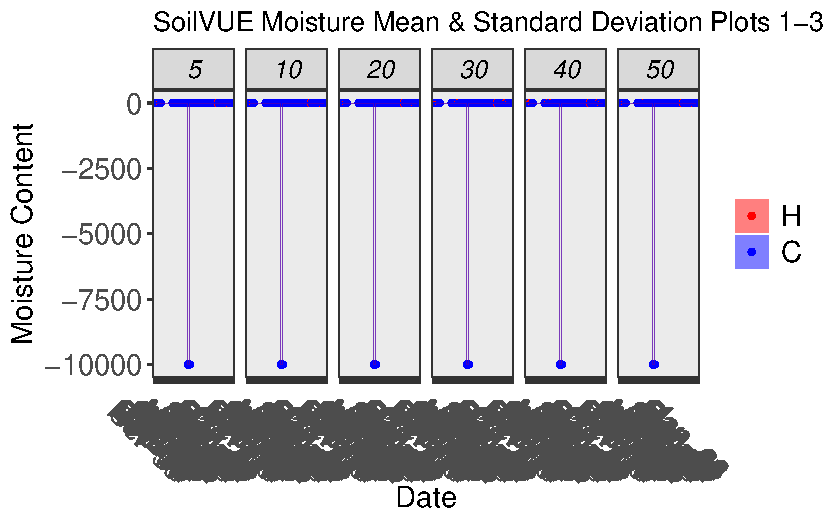
\includegraphics[keepaspectratio]{SVtilden_Code_emmaedit_files/figure-pdf/unnamed-chunk-18-3.pdf}}

\begin{Shaded}
\begin{Highlighting}[]
\CommentTok{\#SoilVUE Electrical Conductivity}
\NormalTok{EC.sv}\OtherTok{\textless{}{-}} \FunctionTok{subset}\NormalTok{(sv, measurement}\SpecialCharTok{==}\StringTok{"EC"}\NormalTok{)}


\NormalTok{EC.sv}\SpecialCharTok{$}\NormalTok{PP}\OtherTok{\textless{}{-}} \FunctionTok{as.numeric}\NormalTok{(EC.sv}\SpecialCharTok{$}\NormalTok{PP)}

\FunctionTok{unique}\NormalTok{(EC.sv}\SpecialCharTok{$}\NormalTok{depth)}
\end{Highlighting}
\end{Shaded}

\begin{verbatim}
[1] "05cm" "10cm" "20cm" "30cm" "40cm" "50cm"
\end{verbatim}

\begin{Shaded}
\begin{Highlighting}[]
\NormalTok{EC.sv}\SpecialCharTok{$}\NormalTok{depth }\OtherTok{\textless{}{-}} \FunctionTok{factor}\NormalTok{(EC.sv}\SpecialCharTok{$}\NormalTok{depth, }\AttributeTok{labels=}\FunctionTok{c}\NormalTok{(}\StringTok{"5 cm"}\NormalTok{, }\StringTok{"10 cm"}\NormalTok{, }\StringTok{"20 cm"}\NormalTok{,}\StringTok{"30 cm"}\NormalTok{, }\StringTok{"40 cm"}\NormalTok{,}\StringTok{"50 cm"}\NormalTok{))}


\CommentTok{\#KEEP}
\CommentTok{\# EC H and C (raw)}
\FunctionTok{ggplot}\NormalTok{(EC.sv, }\FunctionTok{aes}\NormalTok{(}\AttributeTok{x=}\NormalTok{TIMESTAMP, }\AttributeTok{y=}\NormalTok{num, }\AttributeTok{colour=}\NormalTok{trt)) }\SpecialCharTok{+}
  \FunctionTok{geom\_point}\NormalTok{(}\AttributeTok{size=}\FloatTok{0.5}\NormalTok{) }\SpecialCharTok{+} 
  \FunctionTok{ylab}\NormalTok{(}\FunctionTok{expression}\NormalTok{(}\StringTok{"Electrical Conductivity (dS/m)"}\NormalTok{)) }\SpecialCharTok{+}
  \FunctionTok{xlab}\NormalTok{(}\StringTok{"Date"}\NormalTok{) }\SpecialCharTok{+}
  \FunctionTok{scale\_color\_manual}\NormalTok{(}\AttributeTok{values =} \FunctionTok{c}\NormalTok{(}\StringTok{"C"} \OtherTok{=} \StringTok{"blue"}\NormalTok{, }\StringTok{"H"} \OtherTok{=} \StringTok{"red"}\NormalTok{)) }\SpecialCharTok{+}
  \FunctionTok{scale\_x\_datetime}\NormalTok{(}
    \AttributeTok{date\_breaks =} \StringTok{"20 days"}\NormalTok{,       }\CommentTok{\# Set break intervals to 20 days}
    \AttributeTok{date\_labels =} \StringTok{"\%d \%b"}       \CommentTok{\# Format the date labels}
\NormalTok{  ) }\SpecialCharTok{+}
  \FunctionTok{ggtitle}\NormalTok{(}\StringTok{"SoilVUE Electrical Conductivity Plots 1{-}3"}\NormalTok{) }\SpecialCharTok{+}
  \FunctionTok{theme\_bw}\NormalTok{() }\SpecialCharTok{+}
  \FunctionTok{theme}\NormalTok{(}
    \AttributeTok{legend.text =} \FunctionTok{element\_text}\NormalTok{(}\AttributeTok{size=}\DecValTok{14}\NormalTok{),}
    \AttributeTok{axis.text.x =} \FunctionTok{element\_text}\NormalTok{(}\AttributeTok{size=} \DecValTok{14}\NormalTok{),}
    \AttributeTok{axis.text.y =} \FunctionTok{element\_text}\NormalTok{(}\AttributeTok{size =} \DecValTok{14}\NormalTok{),}
    \AttributeTok{axis.title.x =} \FunctionTok{element\_text}\NormalTok{(}\AttributeTok{size=}\DecValTok{14}\NormalTok{),  }\CommentTok{\# Increase x{-}axis label font size}
    \AttributeTok{axis.title.y =} \FunctionTok{element\_text}\NormalTok{(}\AttributeTok{size=}\DecValTok{14}\NormalTok{),}\CommentTok{\# Increase y{-}axis label font size}
    \AttributeTok{strip.text =} \FunctionTok{element\_text}\NormalTok{(}\AttributeTok{size =} \DecValTok{12}\NormalTok{, }\AttributeTok{color =} \StringTok{"black"}\NormalTok{, }\AttributeTok{face =} \StringTok{"italic"}\NormalTok{)}
\NormalTok{  ) }\SpecialCharTok{+}
  \FunctionTok{guides}\NormalTok{(}\AttributeTok{colour =} \FunctionTok{guide\_legend}\NormalTok{(}\AttributeTok{title =} \ConstantTok{NULL}\NormalTok{)) }\SpecialCharTok{+}
  \FunctionTok{facet\_grid}\NormalTok{(PP}\SpecialCharTok{\textasciitilde{}}\NormalTok{depth)}
\end{Highlighting}
\end{Shaded}

\begin{verbatim}
Warning: Removed 2597 rows containing missing values or values outside the scale range
(`geom_point()`).
\end{verbatim}

\pandocbounded{\includegraphics[keepaspectratio]{SVtilden_Code_emmaedit_files/figure-pdf/unnamed-chunk-18-4.pdf}}

\begin{Shaded}
\begin{Highlighting}[]
\NormalTok{summary.EC2 }\OtherTok{\textless{}{-}}\NormalTok{ EC.sv }\SpecialCharTok{\%\textgreater{}\%}
\NormalTok{  dplyr}\SpecialCharTok{::}\FunctionTok{group\_by}\NormalTok{(TIMESTAMP,depth, trt) }\SpecialCharTok{\%\textgreater{}\%}
\NormalTok{  dplyr}\SpecialCharTok{::}\FunctionTok{summarise}\NormalTok{(}
    \AttributeTok{N=}\FunctionTok{length}\NormalTok{(num),}
    \AttributeTok{mean=} \FunctionTok{mean}\NormalTok{(num, }\AttributeTok{na.rm=}\NormalTok{T),}
    \AttributeTok{sd=}\FunctionTok{sd}\NormalTok{(num, }\AttributeTok{na.rm=}\NormalTok{T),}
    \AttributeTok{se=}\FunctionTok{sd}\NormalTok{(num, }\AttributeTok{na.rm=}\NormalTok{T)}\SpecialCharTok{/}\FunctionTok{sqrt}\NormalTok{(}\FunctionTok{sum}\NormalTok{(}\SpecialCharTok{!}\FunctionTok{is.na}\NormalTok{(num))))}
\end{Highlighting}
\end{Shaded}

\begin{verbatim}
`summarise()` has grouped output by 'TIMESTAMP', 'depth'. You can override
using the `.groups` argument.
\end{verbatim}

\begin{Shaded}
\begin{Highlighting}[]
\CommentTok{\#KEEP}
\CommentTok{\#Standard deviation all depths}
\FunctionTok{ggplot}\NormalTok{(summary.EC2, }\FunctionTok{aes}\NormalTok{(}\AttributeTok{x =}\NormalTok{ TIMESTAMP, }\AttributeTok{y =}\NormalTok{ mean, }\AttributeTok{colour =}\NormalTok{ trt)) }\SpecialCharTok{+}
  \FunctionTok{geom\_point}\NormalTok{(}\AttributeTok{size =} \DecValTok{1}\NormalTok{) }\SpecialCharTok{+}
  \FunctionTok{geom\_ribbon}\NormalTok{(}\FunctionTok{aes}\NormalTok{(}\AttributeTok{ymin =}\NormalTok{ mean }\SpecialCharTok{{-}}\NormalTok{ sd, }\AttributeTok{ymax =}\NormalTok{ mean }\SpecialCharTok{+}\NormalTok{ sd, }\AttributeTok{fill =}\NormalTok{ trt), }\AttributeTok{alpha =} \FloatTok{0.5}\NormalTok{, }\AttributeTok{colour =} \ConstantTok{NA}\NormalTok{) }\SpecialCharTok{+}
  \FunctionTok{scale\_color\_manual}\NormalTok{(}\AttributeTok{values =} \FunctionTok{c}\NormalTok{(}\StringTok{"C"} \OtherTok{=} \StringTok{"blue"}\NormalTok{, }\StringTok{"H"} \OtherTok{=} \StringTok{"red"}\NormalTok{)) }\SpecialCharTok{+}
  \FunctionTok{scale\_fill\_manual}\NormalTok{(}\AttributeTok{values =} \FunctionTok{c}\NormalTok{(}\StringTok{"C"} \OtherTok{=} \StringTok{"blue"}\NormalTok{, }\StringTok{"H"} \OtherTok{=} \StringTok{"red"}\NormalTok{)) }\SpecialCharTok{+}
  \FunctionTok{ylab}\NormalTok{(}\StringTok{"Electrical Conductivity (dS/m)"}\NormalTok{) }\SpecialCharTok{+}
  \FunctionTok{xlab}\NormalTok{(}\StringTok{"Date"}\NormalTok{) }\SpecialCharTok{+}
  \FunctionTok{theme\_bw}\NormalTok{() }\SpecialCharTok{+}
  \FunctionTok{theme}\NormalTok{(}
    \AttributeTok{legend.text =} \FunctionTok{element\_text}\NormalTok{(}\AttributeTok{size=}\DecValTok{14}\NormalTok{),}
    \AttributeTok{axis.text.x =} \FunctionTok{element\_text}\NormalTok{(}\AttributeTok{size=} \DecValTok{14}\NormalTok{),}
    \AttributeTok{axis.text.y =} \FunctionTok{element\_text}\NormalTok{(}\AttributeTok{size =} \DecValTok{14}\NormalTok{),}
    \AttributeTok{axis.title.x =} \FunctionTok{element\_text}\NormalTok{(}\AttributeTok{size=}\DecValTok{14}\NormalTok{),  }\CommentTok{\# Increase x{-}axis label font size}
    \AttributeTok{axis.title.y =} \FunctionTok{element\_text}\NormalTok{(}\AttributeTok{size=}\DecValTok{14}\NormalTok{),}\CommentTok{\# Increase y{-}axis label font size}
    \AttributeTok{strip.text =} \FunctionTok{element\_text}\NormalTok{(}\AttributeTok{size =} \DecValTok{12}\NormalTok{, }\AttributeTok{color =} \StringTok{"black"}\NormalTok{, }\AttributeTok{face =} \StringTok{"italic"}\NormalTok{)}
\NormalTok{  ) }\SpecialCharTok{+}
  \FunctionTok{facet\_grid}\NormalTok{(}\SpecialCharTok{\textasciitilde{}}\NormalTok{depth) }\SpecialCharTok{+}
  \FunctionTok{ggtitle}\NormalTok{(}\StringTok{"SoilVUE Electrical Conductivity Mean \& Standard Deviation Plots 1{-}3"}\NormalTok{) }\SpecialCharTok{+}
  \FunctionTok{scale\_x\_datetime}\NormalTok{(}\AttributeTok{breaks =} \StringTok{"8 days"}\NormalTok{, }\AttributeTok{date\_labels =} \StringTok{"\%b{-}\%d"}\NormalTok{) }\SpecialCharTok{+}
  \FunctionTok{theme}\NormalTok{(}\AttributeTok{axis.text.x =} \FunctionTok{element\_text}\NormalTok{(}\AttributeTok{angle =} \SpecialCharTok{{-}}\DecValTok{45}\NormalTok{)) }\SpecialCharTok{+}
  \FunctionTok{labs}\NormalTok{(}\AttributeTok{color =} \ConstantTok{NULL}\NormalTok{, }\AttributeTok{fill =} \ConstantTok{NULL}\NormalTok{)}
\end{Highlighting}
\end{Shaded}

\begin{verbatim}
Warning: Removed 12 rows containing missing values or values outside the scale range
(`geom_point()`).
\end{verbatim}

\begin{verbatim}
Warning: Removed 12 rows containing missing values or values outside the scale range
(`geom_ribbon()`).
\end{verbatim}

\pandocbounded{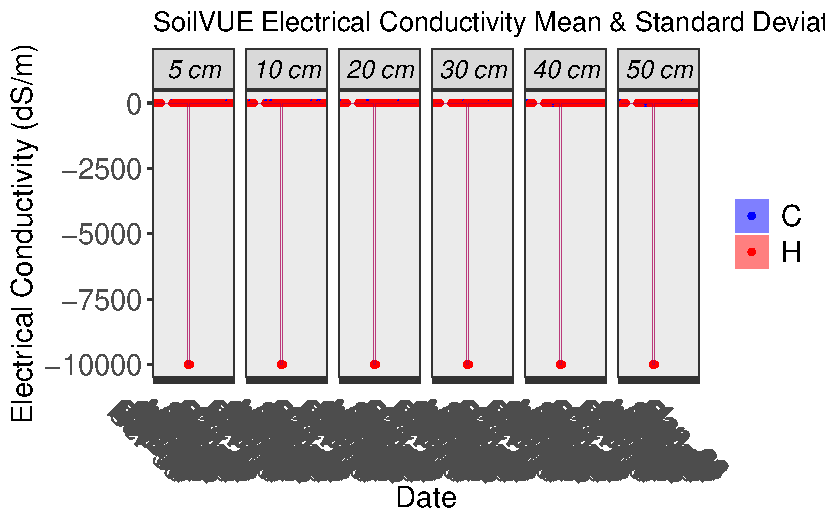
\includegraphics[keepaspectratio]{SVtilden_Code_emmaedit_files/figure-pdf/unnamed-chunk-18-5.pdf}}

\begin{Shaded}
\begin{Highlighting}[]
\CommentTok{\#SoilVUE Permitivity}
\NormalTok{PER.sv}\OtherTok{\textless{}{-}} \FunctionTok{subset}\NormalTok{(sv, measurement}\SpecialCharTok{==}\StringTok{"permitivity"}\NormalTok{)}


\NormalTok{PER.sv}\SpecialCharTok{$}\NormalTok{PP}\OtherTok{\textless{}{-}} \FunctionTok{as.numeric}\NormalTok{(PER.sv}\SpecialCharTok{$}\NormalTok{PP)}

\FunctionTok{unique}\NormalTok{(PER.sv}\SpecialCharTok{$}\NormalTok{depth)}
\end{Highlighting}
\end{Shaded}

\begin{verbatim}
[1] "05cm" "10cm" "20cm" "30cm" "40cm" "50cm"
\end{verbatim}

\begin{Shaded}
\begin{Highlighting}[]
\NormalTok{PER.sv}\SpecialCharTok{$}\NormalTok{depth }\OtherTok{\textless{}{-}} \FunctionTok{factor}\NormalTok{(PER.sv}\SpecialCharTok{$}\NormalTok{depth, }\AttributeTok{labels=}\FunctionTok{c}\NormalTok{(}\StringTok{"5 cm"}\NormalTok{, }\StringTok{"10 cm"}\NormalTok{, }\StringTok{"20 cm"}\NormalTok{,}\StringTok{"30 cm"}\NormalTok{, }\StringTok{"40 cm"}\NormalTok{,}\StringTok{"50 cm"}\NormalTok{))}


\CommentTok{\#KEEP}
\CommentTok{\# EC H and C (raw)}
\FunctionTok{ggplot}\NormalTok{(PER.sv, }\FunctionTok{aes}\NormalTok{(}\AttributeTok{x=}\NormalTok{TIMESTAMP, }\AttributeTok{y=}\NormalTok{num, }\AttributeTok{colour=}\NormalTok{trt)) }\SpecialCharTok{+}
  \FunctionTok{geom\_point}\NormalTok{(}\AttributeTok{size=}\FloatTok{0.5}\NormalTok{) }\SpecialCharTok{+} 
  \FunctionTok{ylab}\NormalTok{(}\FunctionTok{expression}\NormalTok{(}\StringTok{"Permittivity (ɛ)"}\NormalTok{)) }\SpecialCharTok{+}
  \FunctionTok{xlab}\NormalTok{(}\StringTok{"Date"}\NormalTok{) }\SpecialCharTok{+}
  \FunctionTok{scale\_color\_manual}\NormalTok{(}\AttributeTok{values =} \FunctionTok{c}\NormalTok{(}\StringTok{"C"} \OtherTok{=} \StringTok{"blue"}\NormalTok{, }\StringTok{"H"} \OtherTok{=} \StringTok{"red"}\NormalTok{)) }\SpecialCharTok{+}
  \FunctionTok{scale\_x\_datetime}\NormalTok{(}
    \AttributeTok{date\_breaks =} \StringTok{"20 days"}\NormalTok{,       }\CommentTok{\# Set break intervals to 20 days}
    \AttributeTok{date\_labels =} \StringTok{"\%d \%b"}       \CommentTok{\# Format the date labels}
\NormalTok{  ) }\SpecialCharTok{+}
  \FunctionTok{ggtitle}\NormalTok{(}\StringTok{"SoilVUE Permittivity Plots 1{-}3"}\NormalTok{) }\SpecialCharTok{+}
  \FunctionTok{theme\_bw}\NormalTok{() }\SpecialCharTok{+}
  \FunctionTok{theme}\NormalTok{(}
    \AttributeTok{legend.text =} \FunctionTok{element\_text}\NormalTok{(}\AttributeTok{size=}\DecValTok{14}\NormalTok{),}
    \AttributeTok{axis.text.x =} \FunctionTok{element\_text}\NormalTok{(}\AttributeTok{size=} \DecValTok{14}\NormalTok{),}
    \AttributeTok{axis.text.y =} \FunctionTok{element\_text}\NormalTok{(}\AttributeTok{size =} \DecValTok{14}\NormalTok{),}
    \AttributeTok{axis.title.x =} \FunctionTok{element\_text}\NormalTok{(}\AttributeTok{size=}\DecValTok{14}\NormalTok{),  }\CommentTok{\# Increase x{-}axis label font size}
    \AttributeTok{axis.title.y =} \FunctionTok{element\_text}\NormalTok{(}\AttributeTok{size=}\DecValTok{14}\NormalTok{),}\CommentTok{\# Increase y{-}axis label font size}
    \AttributeTok{strip.text =} \FunctionTok{element\_text}\NormalTok{(}\AttributeTok{size =} \DecValTok{12}\NormalTok{, }\AttributeTok{color =} \StringTok{"black"}\NormalTok{, }\AttributeTok{face =} \StringTok{"italic"}\NormalTok{)}
\NormalTok{  ) }\SpecialCharTok{+}
  \FunctionTok{guides}\NormalTok{(}\AttributeTok{colour =} \FunctionTok{guide\_legend}\NormalTok{(}\AttributeTok{title =} \ConstantTok{NULL}\NormalTok{)) }\SpecialCharTok{+}
  \FunctionTok{facet\_grid}\NormalTok{(PP}\SpecialCharTok{\textasciitilde{}}\NormalTok{depth)}
\end{Highlighting}
\end{Shaded}

\begin{verbatim}
Warning: Removed 2593 rows containing missing values or values outside the scale range
(`geom_point()`).
\end{verbatim}

\pandocbounded{\includegraphics[keepaspectratio]{SVtilden_Code_emmaedit_files/figure-pdf/unnamed-chunk-18-6.pdf}}

\begin{Shaded}
\begin{Highlighting}[]
\CommentTok{\#  ggsave("C:/Program Files/RStudio/Task 5 Microwarming/Plots/SoilVUE Moisture Plots 1{-}3.pdf", width=15, height=10)}
 \CommentTok{\# ggsave("C:/Program Files/RStudio/Task 5 Microwarming/Plots/Research Paper/SoilVUE Permittivity Plots 1{-}3.jpg", width=15, height=10)}
\end{Highlighting}
\end{Shaded}





\end{document}
